\chapter{De Basis van een Digitaal Ontwerp}
\label{ch:basis}
\chplab{basis}
\chapterquote{Eva werd niet als een soort accessoire van Adam geschapen, maar Adam was het eerste ontwerp voor Eva.}{Jeanne Moreau, Frans actrice (1928-)}
\begin{chapterintro}
Zoals de naam van deze cursus reeds doet vermoeden werken we met digitale schakelingen, digitale schakelingen onderscheiden zich van de traditionele analoge schakelingen omdat ze slechts een beperkt aantal waarden kunnen aannemen. In de praktijk werken we bijna uitsluitend met \termen{binaire signalen}. Deze waarden hoeven niet noodzakelijk een verschil in spanning aan te duiden. Sterker nog, het gebruik van elektronica is zelfs niet verplicht. Zo zouden we ook een verschil in stroomsterkte, druk, reflectie,... als parameter kunnen nemen. Het komt er enkel op aan om twee waarden te defini\"eren die we symbolisch zullen voorstellen als 0 en 1 en een reeks operaties te kunnen realiseren voor deze natuurfenomenen. Indien we echter meer dan twee verschillende waarden nodig hebben, kunnen we dit probleem oplossen door een aantal binaire waarden te groeperen. In dit eerste hoofdstuk zullen we een beperkte set aan basisoperaties op deze binaire signalen introduceren: de NOT, AND en OR. We formaliseren deze operaties in de booleaanse algebra. Ook bespreken we een methode om een booleaanse functie te synthetiseren. Tot slot bespreken we het verloop van een digitaal ontwerp en introduceren we een taal om hardware mee te beschrijven: VHDL.
\end{chapterintro}
\minitoc[n]
\section{Logische schakelingen}
\paragraph{}
Het definieren van binaire waarden op zich heeft niet veel nut: we willen met deze binaire waarden bepaalde operaties uitvoeren. Om berekeningen te kunnen uitvoeren maken we gebruik van \termen{logische schakelingen}. Logische schakelingen zijn een reeks operaties op \'e\'en of meer binaire parameters die resulteren in een uitgang. De waarde die op de uitgang staat is hierbij afhankelijk van de ingangen. De set van \gtermen{basisoperaties}{Set van operaties waaruit andere operaties zijn opgebouwd: in de booleaanse algebra zijn dit de NOT, AND en OR.} dient klein, simpel en tegelijk universi\"eel te zijn: elke complexe schakeling moet uit een combinatie van deze basisschakelingen kunnen worden opgebouwd.
\paragraph{}
Als basisschakelingen definieert men meestal de \gtermen{NOT}{Een populaire bassischakeling die $0$ afbeelt op $1$; en $1$ op $0$.}, \gtermen{AND}{Een populaire basisschakeling met twee ingangen. $\tupl{0,0}$, $\tupl{0,1}$ en $\tupl{1,0}$ worden afgebeeld op $0$; en $\tupl{1,1}$ wordt afgebeeld op $1$.} en \gtermen{OR}{Een populaire basisschakeling met twee ingangen. $\tupl{0,0}$ wordt afgebeeld op $0$; en $\tupl{0,1}$, $\tupl{1,0}$ en $\tupl{1,1}$ worden afgebeeld op $1$.} operaties. Deze operaties zijn eenvoudig en gemakkelijk te begrijpen en onthouden. Hoewel booleaanse algebra in heel wat andere cursussen reeds aan bod komt, zullen we er ook in deze cursus enkele secties aan besteden. We zullen de booleaanse algebra behandelen aan de hand van een model met lichtschakelaars.
\subsection{Logische schakelingen in huis}
We beschouwen een schakeling zoals op \figref{switchLight}.
\importtikzfigure{switchLight}{Basis van het lamp-model.}
Zoals we zien zal indien we de schakelaar $x$ indrukken, het lichtje branden. Indien we vervolgens de schakelaar loslaten zien we dat het lampje opnieuw dooft. We formaliseren dit door te schrijven:
\begin{equation}
L=x
\end{equation}
Waarbij we $L$ beschouwen als het al dan niet branden van het lampje, en $x$ aanduidt of de schakelaar al dan niet ingedrukt is. Indien we nu als ingang beschouwen of de schakelaar al dan niet ingedrukt is, en als uitgang of het lichtje al dan niet brandt, kunnen we hiermee functies gaan defini\"eren.
\paragraph{Not}
Indien we de implementatie van de schakelaar aanpassen zijn we in staat om een NOT poort te bouwen. Zoals op \figref{switchLightBasicGatesNot}. Deze schakelaar laat stroom door indien deze niet ingedrukt is. Bijgevolg kunnen we stellen dat het al dan niet branden van het lampje equivalent is met niet de schakelaar indrukken. We formaliseren dit als:
\begin{equation}
L=x'=\neg x=!x=\overline{x}=\mbox{NOT }x
\end{equation}
Zoals we zien zijn er in de loop der tijd nogal wat notaties ingevoerd; wat bovendien eigen is aan de volledige booleaanse algebra. In deze cursus zullen we enkel het accent ($x'$) als negatie gebruiken. Literatuur buiten deze cursus kan echter andere standaarden gebruiken. Een NOT poort wordt vaak ook een \termen{inverter} genoemd.
\paragraph{And}
Soms willen we dat het lampje pas gaat branden indien twee of meer schakelaars allemaal ingedrukt zijn. In dat geval spreken we van een AND. Een AND kunnen we implementeren volgens het lamp-model zoals in \figref{switchLightBasicGatesAnd}. We noteren:
\begin{equation}
L=x\cdot y=x\mbox{ AND }y
\end{equation}
\paragraph{Or}
Een andere basisbewerking is de OR. Hierbij willen we dat het lampje brandt bij minstens \'e\'en ingedrukte schakelaar. Of we noteren:
\begin{equation}
L=x+y=x\mbox{ OR } y
\end{equation}
Een implementatie in het lamp-model is te vinden op \figref{switchLightBasicGatesOr}.
\begin{figure}[htb]
\centering
\subfigure[Not]{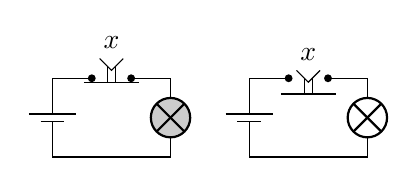
\begin{tikzpicture}
\draw[thick] (-0.3,0.05) -- (0.3,0.05);
\draw (-0.15,-0.05) -- (0.15,-0.05);
\draw (0,0.05) -- (0,0.5) -- (0.5,0.5);
\fill (0.5,0.5) circle (0.05);
\fill (1,0.5) circle (0.05);
\draw (1,0.5) -- (1.5,0.5) -- (1.5,0.25);
\fill[black!20] (1.5,0) circle (0.25);
\draw[thick] (1.5,0) circle (0.25);
\draw[thick] (1.677,0.177) -- (1.323,-0.177);
\draw[thick] (1.677,-0.177) -- (1.323,0.177);
\draw (0,-0.05) -- (0,-0.5) -- (1.5,-0.5) -- (1.5,-0.25);
\draw (0.4,0.45) -- (1.1,0.45);
\draw (0.7,0.45) -- (0.7,0.65);
\draw (0.8,0.45) -- (0.8,0.65);
\draw (0.6,0.75) -- (0.75,0.6) -- (0.9,0.75);
\draw (0.75,0.75) node[anchor=south]{$x$};
\begin{scope}[xshift=2.5 cm]
\draw[thick] (-0.3,0.05) -- (0.3,0.05);
\draw (-0.15,-0.05) -- (0.15,-0.05);
\draw (0,0.05) -- (0,0.5) -- (0.5,0.5);
\fill (0.5,0.5) circle (0.05);
\fill (1,0.5) circle (0.05);
\draw (1,0.5) -- (1.5,0.5) -- (1.5,0.25);
\draw[thick] (1.5,0) circle (0.25);
\draw[thick] (1.677,0.177) -- (1.323,-0.177);
\draw[thick] (1.677,-0.177) -- (1.323,0.177);
\draw (0,-0.05) -- (0,-0.5) -- (1.5,-0.5) -- (1.5,-0.25);
\begin{scope}[yshift=-0.15 cm]
\draw (0.4,0.45) -- (1.1,0.45);
\draw (0.7,0.45) -- (0.7,0.65);
\draw (0.8,0.45) -- (0.8,0.65);
\draw (0.6,0.75) -- (0.75,0.6) -- (0.9,0.75);
\draw (0.75,0.75) node[anchor=south]{$x$};
\end{scope}
\end{scope}
\end{tikzpicture}
\figlab{switchLightBasicGatesNot}
}\\
\subfigure[And]{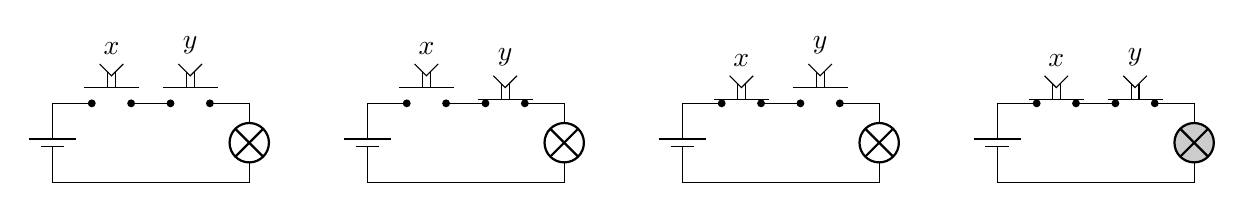
\begin{tikzpicture}
\draw[thick] (-0.3,0.05) -- (0.3,0.05);
\draw (-0.15,-0.05) -- (0.15,-0.05);
\draw (0,0.05) -- (0,0.5) -- (0.5,0.5);
\fill (0.5,0.5) circle (0.05);
\fill (1,0.5) circle (0.05);
\draw (1,0.5) -- (1.5,0.5);
\fill (1.5,0.5) circle (0.05);
\fill (2,0.5) circle (0.05);
\draw (2,0.5) -- (2.5,0.5) -- (2.5,0.25);
\draw[thick] (2.5,0) circle (0.25);
\draw[thick] (2.677,0.177) -- (2.323,-0.177);
\draw[thick] (2.677,-0.177) -- (2.323,0.177);
\draw (0,-0.05) -- (0,-0.5) -- (2.5,-0.5) -- (2.5,-0.25);
\begin{scope}[yshift=0.25 cm]
\draw (0.4,0.45) -- (1.1,0.45);
\draw (0.7,0.45) -- (0.7,0.65);
\draw (0.8,0.45) -- (0.8,0.65);
\draw (0.6,0.75) -- (0.75,0.6) -- (0.9,0.75);
\draw (0.75,0.75) node[anchor=south]{$x$};
\end{scope}
\begin{scope}[xshift=1 cm,yshift=0.25 cm]
\draw (0.4,0.45) -- (1.1,0.45);
\draw (0.7,0.45) -- (0.7,0.65);
\draw (0.8,0.45) -- (0.8,0.65);
\draw (0.6,0.75) -- (0.75,0.6) -- (0.9,0.75);
\draw (0.75,0.75) node[anchor=south]{$y$};
\end{scope}
\begin{scope}[xshift=4 cm]
\draw[thick] (-0.3,0.05) -- (0.3,0.05);
\draw (-0.15,-0.05) -- (0.15,-0.05);
\draw (0,0.05) -- (0,0.5) -- (0.5,0.5);
\fill (0.5,0.5) circle (0.05);
\fill (1,0.5) circle (0.05);
\draw (1,0.5) -- (1.5,0.5);
\fill (1.5,0.5) circle (0.05);
\fill (2,0.5) circle (0.05);
\draw (2,0.5) -- (2.5,0.5) -- (2.5,0.25);
\draw[thick] (2.5,0) circle (0.25);
\draw[thick] (2.677,0.177) -- (2.323,-0.177);
\draw[thick] (2.677,-0.177) -- (2.323,0.177);
\draw (0,-0.05) -- (0,-0.5) -- (2.5,-0.5) -- (2.5,-0.25);
\begin{scope}[yshift=0.25 cm]
\draw (0.4,0.45) -- (1.1,0.45);
\draw (0.7,0.45) -- (0.7,0.65);
\draw (0.8,0.45) -- (0.8,0.65);
\draw (0.6,0.75) -- (0.75,0.6) -- (0.9,0.75);
\draw (0.75,0.75) node[anchor=south]{$x$};
\end{scope}
\begin{scope}[xshift=1 cm,yshift=0.1 cm]
\draw (0.4,0.45) -- (1.1,0.45);
\draw (0.7,0.45) -- (0.7,0.65);
\draw (0.8,0.45) -- (0.8,0.65);
\draw (0.6,0.75) -- (0.75,0.6) -- (0.9,0.75);
\draw (0.75,0.75) node[anchor=south]{$y$};
\end{scope}
\end{scope}
\begin{scope}[xshift=8 cm]
\draw[thick] (-0.3,0.05) -- (0.3,0.05);
\draw (-0.15,-0.05) -- (0.15,-0.05);
\draw (0,0.05) -- (0,0.5) -- (0.5,0.5);
\fill (0.5,0.5) circle (0.05);
\fill (1,0.5) circle (0.05);
\draw (1,0.5) -- (1.5,0.5);
\fill (1.5,0.5) circle (0.05);
\fill (2,0.5) circle (0.05);
\draw (2,0.5) -- (2.5,0.5) -- (2.5,0.25);
\draw[thick] (2.5,0) circle (0.25);
\draw[thick] (2.677,0.177) -- (2.323,-0.177);
\draw[thick] (2.677,-0.177) -- (2.323,0.177);
\draw (0,-0.05) -- (0,-0.5) -- (2.5,-0.5) -- (2.5,-0.25);
\begin{scope}[yshift=0.1 cm]
\draw (0.4,0.45) -- (1.1,0.45);
\draw (0.7,0.45) -- (0.7,0.65);
\draw (0.8,0.45) -- (0.8,0.65);
\draw (0.6,0.75) -- (0.75,0.6) -- (0.9,0.75);
\draw (0.75,0.75) node[anchor=south]{$x$};
\end{scope}
\begin{scope}[xshift=1 cm,yshift=0.25 cm]
\draw (0.4,0.45) -- (1.1,0.45);
\draw (0.7,0.45) -- (0.7,0.65);
\draw (0.8,0.45) -- (0.8,0.65);
\draw (0.6,0.75) -- (0.75,0.6) -- (0.9,0.75);
\draw (0.75,0.75) node[anchor=south]{$y$};
\end{scope}
\end{scope}
\begin{scope}[xshift=12 cm]
\draw[thick] (-0.3,0.05) -- (0.3,0.05);
\draw (-0.15,-0.05) -- (0.15,-0.05);
\draw (0,0.05) -- (0,0.5) -- (0.5,0.5);
\fill (0.5,0.5) circle (0.05);
\fill (1,0.5) circle (0.05);
\draw (1,0.5) -- (1.5,0.5);
\fill (1.5,0.5) circle (0.05);
\fill (2,0.5) circle (0.05);
\draw (2,0.5) -- (2.5,0.5) -- (2.5,0.25);
\fill[black!20] (2.5,0) circle (0.25);
\draw[thick] (2.5,0) circle (0.25);
\draw[thick] (2.677,0.177) -- (2.323,-0.177);
\draw[thick] (2.677,-0.177) -- (2.323,0.177);
\draw (0,-0.05) -- (0,-0.5) -- (2.5,-0.5) -- (2.5,-0.25);
\begin{scope}[yshift=0.1 cm]
\draw (0.4,0.45) -- (1.1,0.45);
\draw (0.7,0.45) -- (0.7,0.65);
\draw (0.8,0.45) -- (0.8,0.65);
\draw (0.6,0.75) -- (0.75,0.6) -- (0.9,0.75);
\draw (0.75,0.75) node[anchor=south]{$x$};
\end{scope}
\begin{scope}[xshift=1 cm,yshift=0.1 cm]
\draw (0.4,0.45) -- (1.1,0.45);
\draw (0.7,0.45) -- (0.7,0.65);
\draw (0.8,0.45) -- (0.8,0.65);
\draw (0.6,0.75) -- (0.75,0.6) -- (0.9,0.75);
\draw (0.75,0.75) node[anchor=south]{$y$};
\end{scope}
\end{scope}
\end{tikzpicture}
\figlab{switchLightBasicGatesAnd}
}\\
\subfigure[Or]{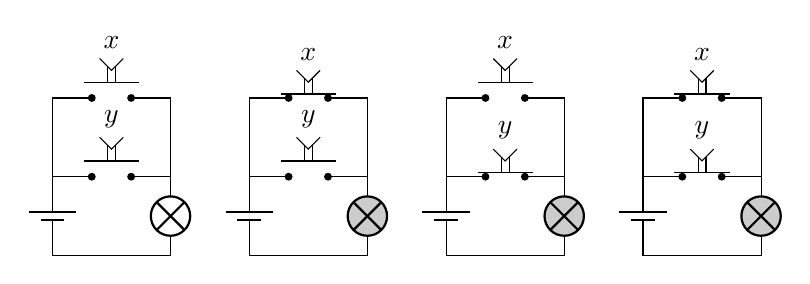
\begin{tikzpicture}
\draw[thick] (-0.3,0.05) -- (0.3,0.05);
\draw (-0.15,-0.05) -- (0.15,-0.05);
\draw (0,0.05) -- (0,0.5) -- (0.5,0.5);
\draw (0,0.5) -- (0,1.5) -- (0.5,1.5);
\fill (0.5,0.5) circle (0.05);
\fill (1,0.5) circle (0.05);
\draw (1,1.5) -- (1.5,1.5) -- (1.5,0.5);
\draw (1,0.5) -- (1.5,0.5) -- (1.5,0.25);
\fill (0.5,1.5) circle (0.05);
\fill (1,1.5) circle (0.05);
\draw[thick] (1.5,0) circle (0.25);
\draw[thick] (1.677,0.177) -- (1.323,-0.177);
\draw[thick] (1.677,-0.177) -- (1.323,0.177);
\draw (0,-0.05) -- (0,-0.5) -- (1.5,-0.5) -- (1.5,-0.25);
\begin{scope}[yshift=0.25 cm]
\draw (0.4,0.45) -- (1.1,0.45);
\draw (0.7,0.45) -- (0.7,0.65);
\draw (0.8,0.45) -- (0.8,0.65);
\draw (0.6,0.75) -- (0.75,0.6) -- (0.9,0.75);
\draw (0.75,0.75) node[anchor=south]{$y$};
\end{scope}
\begin{scope}[yshift=1.25 cm]
\draw (0.4,0.45) -- (1.1,0.45);
\draw (0.7,0.45) -- (0.7,0.65);
\draw (0.8,0.45) -- (0.8,0.65);
\draw (0.6,0.75) -- (0.75,0.6) -- (0.9,0.75);
\draw (0.75,0.75) node[anchor=south]{$x$};
\end{scope}
\begin{scope}[xshift=2.5 cm]
\draw[thick] (-0.3,0.05) -- (0.3,0.05);
\draw (-0.15,-0.05) -- (0.15,-0.05);
\draw (0,0.05) -- (0,0.5) -- (0.5,0.5);
\draw (0,0.5) -- (0,1.5) -- (0.5,1.5);
\fill (0.5,0.5) circle (0.05);
\fill (1,0.5) circle (0.05);
\draw (1,1.5) -- (1.5,1.5) -- (1.5,0.5);
\draw (1,0.5) -- (1.5,0.5) -- (1.5,0.25);
\fill (0.5,1.5) circle (0.05);
\fill (1,1.5) circle (0.05);
\fill[black!20] (1.5,0) circle (0.25);
\draw[thick] (1.5,0) circle (0.25);
\draw[thick] (1.677,0.177) -- (1.323,-0.177);
\draw[thick] (1.677,-0.177) -- (1.323,0.177);
\draw (0,-0.05) -- (0,-0.5) -- (1.5,-0.5) -- (1.5,-0.25);
\begin{scope}[yshift=0.25 cm]
\draw (0.4,0.45) -- (1.1,0.45);
\draw (0.7,0.45) -- (0.7,0.65);
\draw (0.8,0.45) -- (0.8,0.65);
\draw (0.6,0.75) -- (0.75,0.6) -- (0.9,0.75);
\draw (0.75,0.75) node[anchor=south]{$y$};
\end{scope}
\begin{scope}[yshift=1.1 cm]
\draw (0.4,0.45) -- (1.1,0.45);
\draw (0.7,0.45) -- (0.7,0.65);
\draw (0.8,0.45) -- (0.8,0.65);
\draw (0.6,0.75) -- (0.75,0.6) -- (0.9,0.75);
\draw (0.75,0.75) node[anchor=south]{$x$};
\end{scope}
\end{scope}
\begin{scope}[xshift=5 cm]
\draw[thick] (-0.3,0.05) -- (0.3,0.05);
\draw (-0.15,-0.05) -- (0.15,-0.05);
\draw (0,0.05) -- (0,0.5) -- (0.5,0.5);
\draw (0,0.5) -- (0,1.5) -- (0.5,1.5);
\fill (0.5,0.5) circle (0.05);
\fill (1,0.5) circle (0.05);
\draw (1,1.5) -- (1.5,1.5) -- (1.5,0.5);
\draw (1,0.5) -- (1.5,0.5) -- (1.5,0.25);
\fill (0.5,1.5) circle (0.05);
\fill (1,1.5) circle (0.05);
\fill[black!20] (1.5,0) circle (0.25);
\draw[thick] (1.5,0) circle (0.25);
\draw[thick] (1.677,0.177) -- (1.323,-0.177);
\draw[thick] (1.677,-0.177) -- (1.323,0.177);
\draw (0,-0.05) -- (0,-0.5) -- (1.5,-0.5) -- (1.5,-0.25);
\begin{scope}[yshift=0.1 cm]
\draw (0.4,0.45) -- (1.1,0.45);
\draw (0.7,0.45) -- (0.7,0.65);
\draw (0.8,0.45) -- (0.8,0.65);
\draw (0.6,0.75) -- (0.75,0.6) -- (0.9,0.75);
\draw (0.75,0.75) node[anchor=south]{$y$};
\end{scope}
\begin{scope}[yshift=1.25 cm]
\draw (0.4,0.45) -- (1.1,0.45);
\draw (0.7,0.45) -- (0.7,0.65);
\draw (0.8,0.45) -- (0.8,0.65);
\draw (0.6,0.75) -- (0.75,0.6) -- (0.9,0.75);
\draw (0.75,0.75) node[anchor=south]{$x$};
\end{scope}
\end{scope}
\begin{scope}[xshift=7.5 cm]
\draw[thick] (-0.3,0.05) -- (0.3,0.05);
\draw (-0.15,-0.05) -- (0.15,-0.05);
\draw (0,0.05) -- (0,0.5) -- (0.5,0.5);
\draw (0,0.5) -- (0,1.5) -- (0.5,1.5);
\fill (0.5,0.5) circle (0.05);
\fill (1,0.5) circle (0.05);
\draw (1,1.5) -- (1.5,1.5) -- (1.5,0.5);
\draw (1,0.5) -- (1.5,0.5) -- (1.5,0.25);
\fill (0.5,1.5) circle (0.05);
\fill (1,1.5) circle (0.05);
\fill[black!20] (1.5,0) circle (0.25);
\draw[thick] (1.5,0) circle (0.25);
\draw[thick] (1.677,0.177) -- (1.323,-0.177);
\draw[thick] (1.677,-0.177) -- (1.323,0.177);
\draw (0,-0.05) -- (0,-0.5) -- (1.5,-0.5) -- (1.5,-0.25);
\begin{scope}[yshift=0.1 cm]
\draw (0.4,0.45) -- (1.1,0.45);
\draw (0.7,0.45) -- (0.7,0.65);
\draw (0.8,0.45) -- (0.8,0.65);
\draw (0.6,0.75) -- (0.75,0.6) -- (0.9,0.75);
\draw (0.75,0.75) node[anchor=south]{$y$};
\end{scope}
\begin{scope}[yshift=1.1 cm]
\draw (0.4,0.45) -- (1.1,0.45);
\draw (0.7,0.45) -- (0.7,0.65);
\draw (0.8,0.45) -- (0.8,0.65);
\draw (0.6,0.75) -- (0.75,0.6) -- (0.9,0.75);
\draw (0.75,0.75) node[anchor=south]{$x$};
\end{scope}
\end{scope}
\end{tikzpicture}
\figlab{switchLightBasicGatesOr}
}
\caption{Implementatie van de basispoorten volgens het lamp-model.}
\figlab{switchLightBasicGates}
\end{figure}
\paragraph{}
Door deze drie basisbewerkingen met elkaar te combineren kunnen we eindeloos veel nieuwe bewerkingen bouwen. Zoals bijvoorbeeld de exclusieve OR, ook wel de \gtermen{XOR}{Een populaire basisschakeling met twee ingangen. Hierbij worden $\tupl{0,0}$ en $\tupl{1,1}$ afgebeeld op $0$; en $\tupl{0,1}$ en $\tupl{1,0}$ afgebeeld op $1$.} genoemd. De XOR is een bewerking waarbij het lampje gaat branden indien juist \'e\'en van de twee schakelaars ingedrukt is. Deze bewerking kunnen we realiseren door NOT, AND en OR bewerkingen te combineren als volgt:
\begin{equation}
L=x \oplus y=x\mbox{ XOR }y=\left(x\cdot y'\right)+\left(x'\cdot y\right)
\end{equation}
Deze schakelingen kunnen we dan vervolgens in ons lamp-model omzetten zoals op \figref{switchLightXor}.
\begin{figure}[htb]
\centering
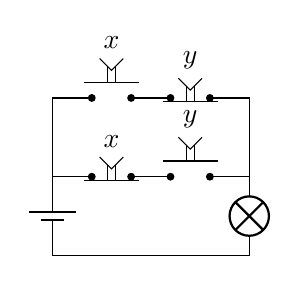
\begin{tikzpicture}
\draw[thick] (-0.3,0.05) -- (0.3,0.05);
\draw (-0.15,-0.05) -- (0.15,-0.05);
\draw (0,0.05) -- (0,0.5) -- (0.5,0.5);
\draw (0,0.5) -- (0,1.5) -- (0.5,1.5);
\fill (0.5,0.5) circle (0.05);
\fill (1,0.5) circle (0.05);
\fill (1.5,0.5) circle (0.05);
\fill (2,0.5) circle (0.05);
\draw (1,1.5) -- (1.5,1.5);
\draw (2,1.5) -- (2.5,1.5) -- (2.5,0.5);
\draw (1,0.5) -- (1.5,0.5);
\draw (2,0.5) -- (2.5,0.5) -- (2.5,0.25);
\fill (0.5,1.5) circle (0.05);
\fill (1,1.5) circle (0.05);
\fill (1.5,1.5) circle (0.05);
\fill (2,1.5) circle (0.05);
\draw[thick] (2.5,0) circle (0.25);
\draw[thick] (2.677,0.177) -- (2.323,-0.177);
\draw[thick] (2.677,-0.177) -- (2.323,0.177);
\draw (0,-0.05) -- (0,-0.5) -- (2.5,-0.5) -- (2.5,-0.25);
\begin{scope}[yshift=0 cm]
\draw (0.4,0.45) -- (1.1,0.45);
\draw (0.7,0.45) -- (0.7,0.65);
\draw (0.8,0.45) -- (0.8,0.65);
\draw (0.6,0.75) -- (0.75,0.6) -- (0.9,0.75);
\draw (0.75,0.75) node[anchor=south]{$x$};
\end{scope}
\begin{scope}[xshift=1cm,yshift=0.25 cm]
\draw (0.4,0.45) -- (1.1,0.45);
\draw (0.7,0.45) -- (0.7,0.65);
\draw (0.8,0.45) -- (0.8,0.65);
\draw (0.6,0.75) -- (0.75,0.6) -- (0.9,0.75);
\draw (0.75,0.75) node[anchor=south]{$y$};
\end{scope}
\begin{scope}[yshift=1.25 cm]
\draw (0.4,0.45) -- (1.1,0.45);
\draw (0.7,0.45) -- (0.7,0.65);
\draw (0.8,0.45) -- (0.8,0.65);
\draw (0.6,0.75) -- (0.75,0.6) -- (0.9,0.75);
\draw (0.75,0.75) node[anchor=south]{$x$};
\end{scope}
\begin{scope}[xshift=1cm,yshift=1 cm]
\draw (0.4,0.45) -- (1.1,0.45);
\draw (0.7,0.45) -- (0.7,0.65);
\draw (0.8,0.45) -- (0.8,0.65);
\draw (0.6,0.75) -- (0.75,0.6) -- (0.9,0.75);
\draw (0.75,0.75) node[anchor=south]{$y$};
\end{scope}
\end{tikzpicture}
\caption{XOR-poort in het lamp-model.}
\figlab{switchLightXor}
\end{figure}
\subsection{Waarheidstabellen}
We kunnen alle schakelingen voorstellen met het lamp-model. Toch is het niet echt praktisch, we gaan dus op zoek naar andere manieren om de logische formules te berekenen, en ook eenvoudig voor te stellen. Een makkelijke manier om logische schakelingen te berekenen is met behulp van \termen{waarheidstabellen}. Een waarheidstabel is een tabel waarbij we alle variabelen voorstellen, en vervolgens met eventuele tussenstappen de uiteindelijke bewerking berekenen. Hierbij maken we gebruik van waarheidstabellen die we reeds kennen: de waarheidstabellen van de basisfuncties.

\paragraph{}
Indien we $n$ variabelen beschouwen betekent dit dat onze waarheidstabel $2^n$ rijen telt. Immers kan elke variabele ofwel $0$ ofwel $1$ zijn. Bovendien is het aantal functies met $n$ variabelen beperkt tot $2^{2^n}$. Dit zegt echter niet over het aantal mogelijke implementaties: deze is onbegrensd. In \tblref{truthTablesBasicGates} geven we de waarheidstabellen van de basisoperaties weer.
\begin{table}[htb]
\centering
\subtable[Not]{
\begin{tabular}{c|c}
$x$&$x'$\\\hline
0&1\\
1&0
\end{tabular}}
\subtable[And]{
\begin{tabular}{cc|c}
$x$&$y$&$x\cdot y$\\\hline
0&0&0\\
0&1&0\\
1&0&0\\
1&1&1
\end{tabular}}
\subtable[Or]{
\begin{tabular}{cc|c}
$x$&$y$&$x+y$\\\hline
0&0&0\\
0&1&1\\
1&0&1\\
1&1&1
\end{tabular}}
\caption{Waarheidstabellen van de basisoperaties.}
\label{tbl:truthTablesBasicGates}
\end{table}
\paragraph{}
We kunnen vervolgens aan de hand van deze waarheidstabellen de werking van een XOR-bewerking bestuderen. We dienen eenvoudigweg basisoperaties toe te passen op deelresultaten om zo uiteindelijk het finale gedrag van de bewerking te kennen zoals in \tblref{truthTableXOR}. Indien twee implementaties voor iedere rij dezelfde uitvoer genereren, zijn de implementaties equivalent, en beschrijven ze dezelfde functie. Equivalente implementaties zijn nuttig om een schakeling effici\"enter te maken. We gaan immers altijd op zoek naar equivalente implementaties die minder kosten of sneller werken.
\begin{table}[htb]
\centering
\begin{tabular}{cc|ccccc|c}
$x$&$y$&$x'$&$y'$&$x'\cdot y$&$x\cdot y'$&$x'\cdot y+x\cdot y'$&$x\oplus y$\\\hline
0&0&1&1&0&0&0&0\\
0&1&1&0&1&0&1&1\\
1&0&0&1&0&1&1&1\\
1&1&0&0&0&0&0&0\\
\end{tabular}
\caption{Waarheidstabel voor de implementatie van een XOR.}
\label{tbl:truthTableXOR}
\end{table}
\subsection{Logische poorten}
\label{ss:logischePoorten}
\ssclab{logischePoorten}
Naast het uitrekenen van operaties heeft ons lamp-model nog een nadeel. Het is erg onpraktisch om grote en complexe schakelingen voor te stellen. Een algemeen geaccepteerde notatie is deze met behulp van \termen{logische poorten}. Poorten zijn kleine componenten die enkele ingangen bevatten, en \'e\'en uitgang. Op figuren \ref{fig:basicGatesNot} tot en met \ref{fig:basicGatesOr} geven we de poorten van de basisbewerkingen weer. We kunnen alle mogelijke schakelingen bouwen met deze poorten. Toch worden vaak ook alternatieve poorten gedefinieerd om veelgebruikte bewerkingen mee toe te passen.

\paragraph{}
Bovendien kunnen we de werking van de basis poorten ook veralgemenen naar meer ingangen. Zo defini\"eren we een \gtermen{$n$-and}{Een basisschakeling met $n$ ingangen. $\tupl{1,1,\ldots,1}$ wordt afgebeeld op $1$; en alle overige configuraties op $0$.} als een poort waar enkel een $1$ op de uitgang verschijnt indien op alle $n$ ingangen een $1$ staat. \figref{basicGatesAndExtended} toont een $3$-and. Een \gtermen{$n$-or}{Een basisschakeling met $n$ ingangen. $\tupl{0,0,\ldots,0}$ wordt afgebeeld op $0$; alle overige configuraties op $1$.} is een poort waar enkel een $0$ op de uitgang verschijnt indien op alle $n$ ingangen een $0$ staat. Zo staat op \figref{basicGatesOrExtended} een $5$-or.
\begin{figure}[htb]
\centering
\subfigure[Not]{\begin{tikzpicture}[circuit logic US]
  \node[not gate] (A) {};
  \draw (A.input -| -1,0) node[anchor=east]{$x$} -- (A.input);
  \draw (A.output) -- ++(1,0) node[anchor=west]{$L$};
\end{tikzpicture}
\figlab{basicGatesNot}
}
\subfigure[And]{\begin{tikzpicture}[circuit logic US]
  \node[and gate] (A) {};
  \draw (A.input 1 -| -1,0) node[anchor=east]{$x$} -- (A.input 1)
        (A.input 2 -| -1,0) node[anchor=east]{$y$} -- (A.input 2);
  \draw (A.output) -- ++(1,0) node[anchor=west]{$L$};
\end{tikzpicture}
\figlab{basicGatesAnd}
}
\subfigure[Or]{\begin{tikzpicture}[circuit logic US]
  \node[or gate] (A) {};
  \draw (A.input 1 -| -1,0) node[anchor=east]{$x$} -- (A.input 1)
        (A.input 2 -| -1,0) node[anchor=east]{$y$} -- (A.input 2);
  \draw (A.output) -- ++(1,0) node[anchor=west]{$L$};
\end{tikzpicture}
\figlab{basicGatesOr}
}
\subfigure[3-and]{\begin{tikzpicture}[circuit logic US]
  \node[and gate,inputs={normal,normal,normal}] (A) {};
  \draw (A.input 1 -| -0.75,0) -- (A.input 1)
        (A.input 2 -| -0.75,0) -- (A.input 2)
	(A.input 3 -| -0.75,0) -- (A.input 3);
  \draw (A.output) -- ++(0.5,0);
\end{tikzpicture}
\figlab{basicGatesAndExtended}
}
\subfigure[5-or]{\begin{tikzpicture}[circuit logic US]
  \node[or gate,inputs={normal,normal,normal,normal,normal}] (A) {};
  \draw (A.input 1 -| -0.75,0) -- (A.input 1)
        (A.input 2 -| -0.75,0) -- (A.input 2)
	(A.input 3 -| -0.75,0) -- (A.input 3)
	(A.input 4 -| -0.75,0) -- (A.input 4)
	(A.input 5 -| -0.75,0) -- (A.input 5);
  \draw (A.output) -- ++(0.5,0);
\end{tikzpicture}
\figlab{basicGatesOrExtended}
}
\caption{Basispoorten en uitbreidingen.}
\figlab{basicGates}
\end{figure}
\paragraph{Complexe poorten}
Complexe poorten die in de loop der tijd een eigen symbool kregen zijn onder meer de \gtermen{NOR}{Een basisschakeling met $2$ ingangen. De configuratie $\tupl{0,0}$ wordt afgebeeld op $1$; de overige configuraties op $0$}, \gtermen{NAND}{Een basisschakeling met $2$ ingangen. De configuratie $\tupl{1,1}$ wordt afgebeeld op $0$; de overige configuraties worden afgebeeld op $1$.} en XOR, deze staan afgebeeld op \figref{complexGates}, samen met een equivalent schema dat uitsluitend uit NOT, AND en OR poorten.
\begin{figure}[htb]
\centering
\subfigure[NAND]{\begin{tikzpicture}[circuit logic US]
  \node[nand gate] (A) at (0.5,0) {};
  \draw (A.input 1 -| -1,0) node[anchor=east]{$x$} -- (A.input 1)
        (A.input 2 -| -1,0) node[anchor=east]{$y$} -- (A.input 2);
  \draw (A.output) -- (2.5,0) node[anchor=west]{$L$};

  \node[and gate] (A2) at (0,1) {};
  \node[not gate] (A3) at (1,1) {};
  \draw (A2.input 1 -| -1,0) node[anchor=east]{$x$} -- (A2.input 1)
        (A2.input 2 -| -1,0) node[anchor=east]{$y$} -- (A2.input 2);
  \draw (A2.output) -- (A3.input);
  \draw (A3.output) -- ++(1,0) node[anchor=west]{$L$};
\end{tikzpicture}
\figlab{complexGatesNand}
}
\subfigure[NOR]{\begin{tikzpicture}[circuit logic US]
  \node[nor gate] (A) at (0.5,0) {};
  \draw (A.input 1 -| -1,0) node[anchor=east]{$x$} -- (A.input 1)
        (A.input 2 -| -1,0) node[anchor=east]{$y$} -- (A.input 2);
  \draw (A.output) -- (2.5,0) node[anchor=west]{$L$};
  \node[or gate] (A2) at (0,1) {};
  \node[not gate] (A3) at (1,1) {};
  \draw (A2.input 1 -| -1,0) node[anchor=east]{$x$} -- (A2.input 1)
        (A2.input 2 -| -1,0) node[anchor=east]{$y$} -- (A2.input 2);
  \draw (A2.output) -- (A3.input);
  \draw (A3.output) -- ++(1,0) node[anchor=west]{$L$};
\end{tikzpicture}
\figlab{complexGatesNor}
}
\subfigure[XOR]{\begin{tikzpicture}[circuit logic US]
  \node[xor gate] (A) at (0,-0.5) {};
  \draw (A.input 1 -| -2.5,0) node[anchor=east]{$x$} -- (A.input 1)
        (A.input 2 -| -2.5,0) node[anchor=east]{$y$} -- (A.input 2);
  \draw (A.output) -- ++(2,0) node[anchor=west]{$L$};
  \node[not gate] (A2) at (-1.5,0.5) {};
  \draw (A2.input -| -2.5,0) node[anchor=east]{$y$} -- (A2.input);
  \node[not gate] (A3) at (-1.5,2.5) {};
  \draw (A3.input -| -2.5,0) node[anchor=east]{$x$} -- (A3.input);
  \node[and gate] (A4) at (0,1) {};
  \draw (A2.output) -- ++(0.375,0) |- (A4.input 2);
  \draw (A3.input -| -1.875,0) |- (A4.input 1);
  \node[and gate] (A5) at (0,2) {};
  \draw (A3.output) -- ++(0.375,0) |- (A5.input 1);
  \draw (A2.input -| -2.125,0) |- (A5.input 2);
  \node[or gate] (A6) at (1.5,1.5) {};
  \draw (A4.output) -- ++(0.5,0) |- (A6.input 2);
  \draw (A5.output) -- ++(0.5,0) |- (A6.input 1);
  \draw (A6.output) -- ++(0.5,0) node[anchor=west]{$L$};
\end{tikzpicture}
\figlab{complexGatesXor}
}
\caption{Complexe poorten.}
\figlab{complexGates}
\end{figure}
De waarheidstabellen van deze complexe poorten staan in subsectie \sscref{appendixComplexePoorten}.
\paragraph{Universi\"ele poorten}
De reden dat NAND en NOR poorten populair zijn komt hoofdzakelijk omdat het \gtermen[universiele poorten]{universi\"ele poorten}{Een poort waarmee men elke functie kan bouwen. In de booleaanse logica komt dit er op neer dat men een NOT en AND moet kunnen bouwen. Voorbeelden van universi\"ele poorten zijn de NAND en NOR.} zijn. Dat betekent dat iedere basispoort kan ge\"implementeerd worden met behulp van NAND of NOR poorten. In \tblref{nandNorUniversal} staan deze implementaties. Bovendien is het realiseren van NAND en NOR poorten in de meeste technologie\"en goedkoper dan het bouwen van AND en OR poorten.
\begin{table}[htb]
\centering
\begin{tabular}{c|c|c|c}
&NOT&AND&OR\\\hline
met NAND&
\begin{tikzpicture}[circuit logic US]
  \node[anchor=east] (I) at (-1,0) {$x$};
  \node[nand gate] (A) at (0,0) {};
  \draw (-1,0) -- (-0.75,0)  |- (A.input 1);
  \draw (-0.75,0)  |- (A.input 2);
  \draw (A.output) -- (0.75,0) node[anchor=west]{$L$};
\end{tikzpicture}
&
\begin{tikzpicture}[circuit logic US]
  %\node[anchor=east] (I) at (-1,0) {$x$};
  \node[nand gate] (A1) at (-1.5,0) {};
  \node[nand gate] (A2) at (0,0) {};
  \draw (A1.output) -- (-0.75,0)  |- (A2.input 1);
  \draw (-0.75,0)  |- (A2.input 2);
  \draw (A1.input 1 -| -2.25,0) node[anchor=east]{$x$} -- (A1.input 1)
        (A1.input 2 -| -2.25,0) node[anchor=east]{$y$} -- (A1.input 2);
  \draw (A2.output) -- (0.75,0) node[anchor=west]{$L$};
\end{tikzpicture}
&
\begin{tikzpicture}[circuit logic US]
  \node[anchor=east] (I) at (-1,0.5) {$x$};
  \node[nand gate] (A) at (0,0.5) {};
  \draw (-1,0.5) -- (-0.75,0.5)  |- (A.input 1);
  \draw (-0.75,0.5)  |- (A.input 2);
  \node[anchor=east] (I2) at (-1,-0.5) {$y$};
  \node[nand gate] (A2) at (0,-0.5) {};
  \draw (-1,-0.5) -- (-0.75,-0.5)  |- (A2.input 1);
  \draw (-0.75,-0.5)  |- (A2.input 2);
  \node[nand gate] (A3) at (1.5,0) {};
  \draw (A3.output) -- (2.25,0) node[anchor=west]{$L$};
  \draw (A.output) -- ++(0.25,0) |- (A3.input 1);
  \draw (A2.output) -- ++(0.25,0) |- (A3.input 2);
\end{tikzpicture}
\\\hline
met NOR&
\begin{tikzpicture}[circuit logic US]
  \node[anchor=east] (I) at (-1,0) {$x$};
  \node[nor gate] (A) at (0,0) {};
  \draw (-1,0) -- (-0.75,0)  |- (A.input 1);
  \draw (-0.75,0)  |- (A.input 2);
  \draw (A.output) -- (0.75,0) node[anchor=west]{$L$};
\end{tikzpicture}
&
\begin{tikzpicture}[circuit logic US]
  \node[anchor=east] (I) at (-1,0.5) {$x$};
  \node[nor gate] (A) at (0,0.5) {};
  \draw (-1,0.5) -- (-0.75,0.5)  |- (A.input 1);
  \draw (-0.75,0.5)  |- (A.input 2);
  \node[anchor=east] (I2) at (-1,-0.5) {$y$};
  \node[nor gate] (A2) at (0,-0.5) {};
  \draw (-1,-0.5) -- (-0.75,-0.5)  |- (A2.input 1);
  \draw (-0.75,-0.5)  |- (A2.input 2);
  \node[nor gate] (A3) at (1.5,0) {};
  \draw (A3.output) -- (2.25,0) node[anchor=west]{$L$};
  \draw (A.output) -- ++(0.25,0) |- (A3.input 1);
  \draw (A2.output) -- ++(0.25,0) |- (A3.input 2);
\end{tikzpicture}
&
\begin{tikzpicture}[circuit logic US]
  %\node[anchor=east] (I) at (-1,0) {$x$};
  \node[nor gate] (A1) at (-1.5,0) {};
  \node[nor gate] (A2) at (0,0) {};
  \draw (A1.output) -- (-0.75,0)  |- (A2.input 1);
  \draw (-0.75,0)  |- (A2.input 2);
  \draw (A1.input 1 -| -2.25,0) node[anchor=east]{$x$} -- (A1.input 1)
        (A1.input 2 -| -2.25,0) node[anchor=east]{$y$} -- (A1.input 2);
  \draw (A2.output) -- (0.75,0) node[anchor=west]{$L$};
\end{tikzpicture}
\end{tabular}
\caption{Implementatie van de basispoorten met behulp van NAND en NOR poorten.}
\label{tbl:nandNorUniversal}
\end{table}
\paragraph{Ge\"inverteerde ingangen}
Tot slot introduceren we nog een andere conventie die vaak gebruikt wordt: \gtermen[geinverteerde ingangen]{ge\"inverteerde ingangen}{Een conventie die wordt gebruikt om het aantal getekende NOT poorten in een schema drastisch te verminderen. Men zet hierbij cirkels  bij de ingangen van een poort. Deze cirkels duiden dan op een invertering (en dus eventueel een NOT poort) voor deze ingang.}. NOT poorten worden heel vaak gebruikt, ook bij ingangen van andere poorten. Het symbool van de NOT poort neemt nogal wat plaats in op een schema. Daardoor is het de gewoonte om soms cirkels te tekenen aan de ingangen van een bepaalde poort: ge\"inverteerde ingangen. Deze cirkels stellen een NOT poort voor. Concrete voorbeelden staan op \figref{basicGatesInvertedInput}. In het algemeen kunnen we dus zeggen dat een cirkel duidt op het inverteren. Inverteren in het schema betekent echter niet noodzakelijk dat we bij de fysische implementatie gebruik moeten maken van een inverter (meestal is het zelfs omgekeerd): men kan vaak de implementatie van de poort zo aanpassen dat er geen extra transistoren nodig zijn voor deze transformatie.
\begin{figure}[htb]
\centering
\subfigure{\begin{tikzpicture}[circuit logic US]
  \node[and gate,inputs={inverted,inverted}] (A) {};
  \draw (A.input 1 -| -0.75,0) -- (A.input 1)
        (A.input 2 -| -0.75,0) -- (A.input 2);
  \draw (A.output) -- ++(0.5,0);
\end{tikzpicture}
}
\subfigure{\begin{tikzpicture}[circuit logic US]
  \node[or gate, inputs={normal,inverted}] (A) {};
  \draw (A.input 1 -| -0.75,0) -- (A.input 1)
        (A.input 2 -| -0.75,0) -- (A.input 2);
  \draw (A.output) -- ++(0.5,0);
\end{tikzpicture}
}
\subfigure{\begin{tikzpicture}[circuit logic US]
  \node[and gate,inputs={normal,normal,inverted}] (A) {};
  \draw (A.input 1 -| -0.75,0) -- (A.input 1)
        (A.input 2 -| -0.75,0) -- (A.input 2)
	(A.input 3 -| -0.75,0) -- (A.input 3);
  \draw (A.output) -- ++(0.5,0);
\end{tikzpicture}
}
\subfigure{\begin{tikzpicture}[circuit logic US]
  \node[or gate,inputs={normal,inverted,inverted,normal,normal}] (A) {};
  \draw (A.input 1 -| -0.75,0) -- (A.input 1)
        (A.input 2 -| -0.75,0) -- (A.input 2)
	(A.input 3 -| -0.75,0) -- (A.input 3)
	(A.input 4 -| -0.75,0) -- (A.input 4)
	(A.input 5 -| -0.75,0) -- (A.input 5);
  \draw (A.output) -- ++(0.5,0);
\end{tikzpicture}
}
\caption{Poorten met ge\"inverteerde ingangen.}
\figlab{basicGatesInvertedInput}
\end{figure}
\subsection{Logische schakelingen}
De vorige subsectie toonde al dat we met deze poorten netwerken kunnen bouwen. Deze netwerken worden \gtermen{logische schakelingen}{Een netwerk van logische poorten.} genoemd. Deze schakelingen implementeren dan uiteindelijk de functionaliteiten waarvoor we een digitaal circuit ontwerpen. We kunnen logische schakelingen beschrijven door middel van een schema zoals we dat tot nu toe altijd gedaan hebben. Een andere techniek is echter op basis van een taal: VHDL\footnote{VHDL: VHSIC Hardware Design Language; VHSIC: Very High Speed Integrated Circuit.}. Deze taal komt onder meer aan bod in sectie \secref{vhdl}, en verder in de verdere hoofdstukken van deze cursus.
\paragraph{Optimaliseren}
Een belangrijk probleem met schakelingen is het vinden van een optimale implementatie voor een bepaalde functie. Sommige schakelingen zijn immers equivalent. Bijgevolg zoeken we voor een probleem uit de set van equivalente schakelingen naar de schakeling die ons het meeste voordeel oplevert. Hiervoor zijn enkele parameters belangrijk: kostprijs en verwerkingskracht. We proberen de kostprijs immers te minimaliseren. De kostprijs is eenvoudig te berekenen met volgende formule:
\begin{equation}
\mbox{Kostprijs}=\mbox{\#poortingangen}+\mbox{\#poortuitgangen}-\mbox{\#inverters}
\label{eqn:kosten}
\end{equation}
Merk op dat deze formule geen eenheid heeft. Het is dan ook niet de bedoeling de kostprijs in bijvoorbeeld euro te berekenen. Het is eerder bedoeld als een ruwe metriek om verschillende schakelingen met elkaar te kunnen vergelijken.
\subparagraph{}
De verwerkingskracht wordt bepaald door het concept van de zwakste schakel. Ketens waarbij de uitgangen van poorten weer nieuwe ingangen aansturen zijn immers nefast. We streven dus naar circuits waarbij een signaal slechts door een beperkt aantal poorten heen moet. De lengte van het langste pad is echter niet makkelijk te berekenen. Immers hangt de vertraging van een poort af van onder meer het type en het aantal ingangen. Het totaal aantal ingangen daarentegen geeft in de meeste gevallen een goede ruwe schatting. We formaliseren tot:
\begin{equation}
\mbox{Minimale vertraging}\propto\mbox{\#poortingangen}%=?
\end{equation}
\paragraph{Tijdsgedrag}In de vorige paragraaf hadden we het reeds over performantie. Snelle systemen worden echter vaak beperkt door het tijdsgedrag van logische schakelingen. Wiskundig gezien levert een verandering aan de ingang immers altijd onmiddellijk een correct signaal aan de uitgang. Maar zoals we reeds gesteld hebben, heeft een poort een zekere tijd nodig om de verandering aan de ingang door te rekenen. Dit lijkt slechts een detail. Een nadelig effect hiervan is echter dat er overgangsverschijnselen kunnen ontstaan. In de eerste plaats omdat een waarde afhangt van twee ketens van poorten. En het veranderde ingangssignaal propageert zich sneller door de ene dan door de andere keten. Aan de andere kant ook omdat men nu eenmaal niet iedere poort uniform kan aanmaken. Tussen twee (dezelfde) poorten kunnen toch kleine tijdsverschillen optreden. In dat geval spreken we van een \termen{glitch}. \figref{timeBehaviorGlitchExample} toont een scenario van veranderende signalen in een logische schakeling met een glitch.
\begin{figure}[htb]
\centering
\begin{tikzpicture}[circuit logic US]
  \node[not gate] (N) at (0,0.5) {};
  \node[and gate] (A) at (0,-0.5) {};
  \node[or gate] (O) at (2,0) {};
  \draw (-1.5,0.5) node[anchor=east]{$x$} -- (N.input);
  \draw (A.input 2 -| -1.5,0) node[anchor=east]{$y$} -- (A.input 2);
  \draw (-1,0.5) |- (A.input 1);
  \draw (N.output) -- (1,0.5) node[anchor=south east]{$a$} |- (O.input 1);
  \draw (A.output) -- (1,-0.5) node[anchor=north east]{$b$} |- (O.input 2);
  \draw (O.output) -- ++(0.5,0) node[anchor=west]{$f$};
  \begin{scope}[xshift=5 cm]
  \draw[thick,->] (0,2) -- (0,-2) -- (6,-2) node[anchor=south east]{$t$};
  \foreach\y in {0,1,...,3} {
    \draw[gray] (-1,-1.2+0.8*\y) -- (6,-1.2+0.8*\y);
    \draw[dashed] (1+\y,-2) -- (1+\y,2);
  }
  \foreach\y/\ty in {0/f,1/b,2/a,3/y,4/x} {
    \draw (-0.5,-1.6+0.8*\y) node[anchor=east]{$\ty$};
    \draw (0,-1.8+0.8*\y) node[anchor=east]{0};
    \draw (0,-1.4+0.8*\y) node[anchor=east]{1};
  }
  \begin{scope}[yshift=1.4 cm,yscale=0.4]
    \draw (0,0) -- (1,0) -- (1,1) -- (3,1) -- (3,0) -- (6,0);
  \end{scope}
  \begin{scope}[yshift=0.6 cm,yscale=0.4]
    \draw (0,0) -- (2,0) -- (2,1) -- (4,1) -- (4,0) -- (6,0);
  \end{scope}
  \begin{scope}[yshift=-0.2 cm,yscale=0.4]%not is lagging 0.2
    \draw (0,1) -- (1.2,1) -- (1.2,0) -- (3.2,0) -- (3.2,1) -- (6,1);
  \end{scope}
  \begin{scope}[yshift=-1 cm,yscale=0.4]%and is lagging 0.1
    \draw (0,0) -- (2.1,0) -- (2.1,1) -- (3.1,1) -- (3.1,0) -- (6,0);
  \end{scope}
  \begin{scope}[yshift=-1.8 cm,yscale=0.4]%or is lagging 0.15
    \draw (0,1) -- (1.35,1) -- (1.35,0) -- (2.25,0) -- (2.25,1) -- (3.25,1) -- (3.25,0) -- (3.35,0) node[anchor=south west,yshift=-0.1 cm]{``glitch''} -- (3.35,1) -- (6,1);
  \end{scope}
  \end{scope}
\end{tikzpicture}
\caption{Voorbeeld van het tijdsgedrag van een logische schakeling met een ``glitch''.}
\figlab{timeBehaviorGlitchExample}
\end{figure}
\section{Booleaanse algebra}
\label{s:booleaanseAlgebra}
De tak van de wiskunde die zich bezighoudt met logische bewerkingen is de \termen{booleaanse algebra}. Deze algebra rekent uitsluitend met de twee logische waarden $\left\{0,1\right\}$ en drie logische operatoren: de ons reeds bekende NOT ($'$), AND ($\cdot$) en OR ($+$). Deze operaties hebben elk een specifieke prioriteit zodat men met een minimum aan haakjes toch een complexe expressie kan beschrijven. Zo heeft de NOT prioriteit op de AND die prioriteit heeft op de OR.\footnote{Een ezelsbruggetje om dit te onthouden is het woord NANO: \underline{N}ot \underline{AN}d \underline{O}r.}
\subsection{Theorema's en eigenschappen}
\label{ss:theoremasPropertiesBooleanAlgebra}
De booleaanse algebra maakt gebruik van theorema's om de operatoren te evalueren. Zo worden de resultaten van logische operatoren zonder variabelen gedefinieerd zoals we dat ook met een waarheidstabel kunnen doen. Deze definities staan in \tblref{booleanAlgebraNone}.
\begin{table}[htb]
\centering
\begin{tabular}{ll}
$0\cdot0=0$&$1+1=1$\\
$1\cdot1=1$&$0+0=0$\\
$0\cdot1=1\cdot0=0$&$1+0=0+1=1$\\
$0'=1$&$1'=0$
\end{tabular}
\caption{Booleaanse algebra zonder variabelen.}
\label{tbl:booleanAlgebraNone}
\end{table}
In de booleaanse algebra wordt ook met variabelen gerekend. Op die manier kan men vaak expressies manipuleren en optimaliseren. Indien we slechts \'e\'en variabele beschouwen gelden regels weergegeven in \tblref{booleanAlgebraSingle}.
\begin{table}[htb]
\centering
\begin{tabular}{ll}
$x\cdot 0=0$&$x+1=1$\\
$x\cdot 1=x$&$x+0=x$\\
$x\cdot x=x$&$x+x=x$\\
$x\cdot x'=0$&$x+x'=1$\\
$(x')'=x$&\\
\end{tabular}
\caption{Booleaanse algebra met \'e\'en variabele.}
\label{tbl:booleanAlgebraSingle}
\end{table}
Tot slot werden ook regels gedefinieerd voor meerdere variabelen. Deze regels kunnen onder meer het aantal variabelen reduceren evenals het aantal operatoren, of tot alternatieve implementaties leiden die mogelijk sneller werken. Een opsomming van deze wetten staan in \tblref{booleanAlgebraMultiple}.
\begin{table}[htb]
\centering
\begin{tabular}{ll}
\multicolumn{2}{c}{\termen{Commutativiteit}}\\
$x\cdot y=y\cdot x$&$x+y=y+x$\\
\multicolumn{2}{c}{\termen{Associativiteit}}\\
$x\cdot (y\cdot z)=(x\cdot y)\cdot z$&$x+(y+z)=(x+y)+z$\\
\multicolumn{2}{c}{\termen{Distributiviteit}}\\
$x\cdot (y+z)=x\cdot y+x\cdot z$&$x+(y\cdot z)=(x+y)\cdot (x+z)$\\
\multicolumn{2}{c}{\termen{Absorptie}}\\
$x+x\cdot y=x$&$x\cdot(x+y)=x$\\
\multicolumn{2}{c}{\termen{Wet van De Morgan}}\\
$(x\cdot y)'=x'+y'$&$(x+y)'=x'\cdot y'$
\end{tabular}
\caption{Booleaanse algebra met meerdere variabelen.}
\label{tbl:booleanAlgebraMultiple}
\end{table}
\paragraph{Dualiteit}Een opmerkelijke eigenschap bij booleaanse algebra is de dualiteit. Indien we bij een van de wetten uit \tblref{booleanAlgebraNone}, \tblref{booleanAlgebraSingle} of \tblref{booleanAlgebraMultiple} de OR operaties door AND operaties vervangen en vice-versa, en de 1 door 0 vervangen en vice-versa, bekomen we eenvoudigweg een andere wet uit deze tabellen. Deze eigenschap noemen we de \termen{dualiteit} van de booleaanse algebra. Bovendien geldt ook dat slechts de helft van de gestelde wetten vereist is. Het andere deel kan met de wetten van De Morgan afgeleid worden.
\paragraph{Verschil met de gewone algebra}Omdat ook de booleaanse algebra een optelling en vermenigvuldiging lijkt te defini\"eren en er bovendien ook analogie\"en te trekken zijn, lijkt het soms dat booleaanse algebra niet verschilt van de standaard algebra. Toch zijn er enkele opmerkelijke verschillen. Zo bestaat er geen verschil of deling in de booleaanse algebra. Verder voldoet in de booleaanse algebra volgend stelsel voor iedere $y$:
\begin{equation}
\left\{\begin{array}{l}
y+y'=1\\
y\cdot y=y
\end{array}\right.
\end{equation}
Terwijl in de standaard algebra er geen enkele $y$ is waarvoor dit geldt. Tot slot is bij standaard algebra de optelling ook niet distributief tegenover de vermenigvuldiging, zo is $5+2\cdot4\neq(5+2)\cdot(5+4)$.
\section{Synthese met logische poorten}
\label{s:synthese}
Nu we weten hoe logische schakelingen werken, en hoe we deze door middel van de booleaanse algebra kunnen uitwerken, wordt het tijd om zelf schakelingen te bouwen. Dit doen we vertrekkend vanuit een waarheidstabel. Soms is het makkelijk om een implementatie af te leiden uit deze waarheidstabellen. Maar indien het aantal variabelen groot wordt of de functie complex is, wordt het vinden van een implementatie moeilijk. In deze cursus stellen we dan ook enkele algemene technieken voor om uit een waarheidstabel een logische functie te genereren. In sectie \ref{s:minimalisatie} zullen we bovendien enkele methodes beschrijven om deze logische implementaties te optimaliseren. Doorheen deze sectie zullen we een logische functie genereren voor de waarheidstabel in \tblref{truthTableExample}.
\begin{table}[htb]
\centering
\begin{tabular}{ccc|c}
$x$&$y$&$z$&$f$\\\hline
0&0&0&0\\
0&0&1&1\\
0&1&0&0\\
0&1&1&0\\
1&0&0&1\\
1&0&1&1\\
1&1&0&1\\
1&1&1&0\\
\end{tabular}
\caption{Waarheidstabel voor het synthese-voorbeeld.}
\label{tbl:truthTableExample}
\end{table}
In de waarheidstabel zien we uitsluitend 0 en 1 staan. In sectie \ref{par:dontcare} zullen we echter kennis maken met een derde toestand: de \termen{don't care}.
\subsection{SOP \& POS}
\termen{Sum-of-Products (SOP)} en \termen{Product-of-Sums (POS)} zijn twee technieken die op een machinale manier uit een waarheidstabel een logische functie genereren. Ze maken respectievelijk gebruik van \termen{mintermen} en \termen{maxtermen}.
\paragraph{Sum-of-Products} De Sum-of-Products maakt gebruik van mintermen. Een minterm is een logische functie die slechts waar is voor \'e\'en gegeven rij in een waarheidstabel. Dit bekomen we door het booleaans product te nemen van alle variabelen. Indien de variabelen negatief zijn wordt de negatie in het product verwerkt. De minterm van rij $i$ noteren we als $m_i$. De Sum-of-Products methode neemt de booleaanse som van \termen{1-mintermen}. Een 1-minterm is een minterm die waar is bij een rij waarbij $f$ ook waar is. \tblref{truthTableExampleMinTerms} toont voor iedere rij de minterm. Wanneer $f$ waar is, wordt ook de 1-minterm ingevuld. Vervolgens bepalen we de som van alle 1-mintermen.
\begin{table}[htb]
\begin{center}
\begin{tabular}{m{0.65\textwidth}|m{0.35\textwidth}}
\begin{center}
\begin{tabular}{ccc|l|c|l}
$x$&$y$&$z$&minterm&$f$&1-minterm\\\hline
0&0&0&$m_0=x'\cdot y'\cdot z'$&0&\\
0&0&1&$m_1=x'\cdot y'\cdot z$&1&$m_1=x'\cdot y'\cdot z$\\
0&1&0&$m_2=x'\cdot y\cdot z'$&0&\\
0&1&1&$m_3=x'\cdot y\cdot z$&0&\\
1&0&0&$m_4=x\cdot y'\cdot z'$&1&$m_4=x\cdot y'\cdot z'$\\
1&0&1&$m_5=x\cdot y'\cdot z$&1&$m_5=x\cdot y'\cdot z$\\
1&1&0&$m_6=x\cdot y\cdot z'$&1&$m_6=x\cdot y\cdot z'$\\
1&1&1&$m_7=x\cdot y\cdot z$&0&\\
\end{tabular}
\end{center}
&
\begin{center}
\begin{tikzpicture}[circuit logic US]
\draw (-2.7,1.7) node[anchor=south]{$x$} -- (-2.7,-1.7);
\draw (-2.5,1.7) node[anchor=south]{$y$} -- (-2.5,-1.7);
\draw (-2.3,1.7) node[anchor=south]{$z$} -- (-2.3,-1.7);

\node[or gate,inputs={normal,normal,normal,normal}] (O) at (0,0) {};
\draw (O.output) -- ++(0.25,0) node[anchor=west]{$f$};

\node[and gate,inputs={inverted,inverted,normal}] (A1) at (-1.5,1.2) {$m_1$};
\draw (A1.output) -- ++(0.35,0) |- (O.input 1);
\draw (A1.input 1 -| -2.7,0) -- (A1.input 1);
\draw (A1.input 2 -| -2.5,0) -- (A1.input 2);
\draw (A1.input 3 -| -2.3,0) -- (A1.input 3);
\node[and gate,inputs={normal,inverted,inverted}] (A4) at (-1.5,0.4) {$m_4$};
\draw (A4.output) -- ++(0.2,0) |- (O.input 2);
\draw (A4.input 1 -| -2.7,0) -- (A4.input 1);
\draw (A4.input 2 -| -2.5,0) -- (A4.input 2);
\draw (A4.input 3 -| -2.3,0) -- (A4.input 3);
\node[and gate,inputs={normal,inverted,normal}] (A5) at (-1.5,-0.4) {$m_5$};
\draw (A5.output) -- ++(0.2,0) |- (O.input 3);
\draw (A5.input 1 -| -2.7,0) -- (A5.input 1);
\draw (A5.input 2 -| -2.5,0) -- (A5.input 2);
\draw (A5.input 3 -| -2.3,0) -- (A5.input 3);
\node[and gate,inputs={normal,normal,inverted}] (A6) at (-1.5,-1.2) {$m_6$};
\draw (A6.output) -- ++(0.35,0) |- (O.input 4);
\draw (A6.input 1 -| -2.7,0) -- (A6.input 1);
\draw (A6.input 2 -| -2.5,0) -- (A6.input 2);
\draw (A6.input 3 -| -2.3,0) -- (A6.input 3);
\end{tikzpicture}
\end{center}
\end{tabular}\\
SOP: $f=m_1+m_4+m_5+m_6=x'\cdot y'\cdot z+x\cdot y'\cdot z'+x\cdot y'\cdot z+x\cdot y\cdot z'$
\end{center}
\caption{Sum-of-Products methode toegepast op het voorbeeld.}
\label{tbl:truthTableExampleMinTerms}
\end{table}
\paragraph{Product-of-Sums} Analoog maakt de Product-of-Sums gebruik van maxtermen. Zoals de naam reeds doet vermoeden is een maxterm een logische functie die altijd waar is behalve voor \'e\'en rij in de waarheidstabel. Indien we de maxterm voor een bepaalde term willen genereren dienen we de booleaanse optelling van de negatie van de variabelen te nemen. We noteren een maxterm voor rij $i$ met $M_i$. De Product-of-Sums methode neemt analoog het booleaanse product van de \termen{0-maxtermen}. Een 0-maxterm is analoog een maxterm wanneer $f$ onwaar is. \tblref{truthTableExampleMaxTerms} toont voor iedere rij de maxterm. Wanneer $f$ onwaar is, wordt ook de 0-maxterm ingevuld. Vervolgens bepalen we het product van alle 0-maxtermen.
\begin{table}[htb]
\begin{center}
\begin{tabular}{m{0.65\textwidth}|m{0.35\textwidth}}
\begin{center}

\begin{tabular}{ccc|l|c|l}
$x$&$y$&$z$&maxterm&$f$&0-maxterm\\\hline
0&0&0&$M_0=x+y+z$&0&$M_0=x+y+z$\\
0&0&1&$M_1=x+y+z'$&1&\\
0&1&0&$M_2=x+y'+z$&0&$M_2=x+y'+z$\\
0&1&1&$M_3=x+y'+z'$&0&$M_3=x+y'+z'$\\
1&0&0&$M_4=x'+y+z$&1&\\
1&0&1&$M_5=x'+y+z'$&1&\\
1&1&0&$M_6=x'+y'+z$&1&\\
1&1&1&$M_7=x'+y'+z'$&0&$M_7=x'+y'+z'$\\
\end{tabular}
\end{center}
&
\begin{center}
\begin{tikzpicture}[circuit logic US]
\draw (-2.7,1.7) node[anchor=south]{$x$} -- (-2.7,-1.7);
\draw (-2.5,1.7) node[anchor=south]{$y$} -- (-2.5,-1.7);
\draw (-2.3,1.7) node[anchor=south]{$z$} -- (-2.3,-1.7);

\node[and gate,inputs={normal,normal,normal,normal}] (O) at (0,0) {};
\draw (O.output) -- ++(0.25,0) node[anchor=west]{$f$};

\node[or gate,inputs={normal,normal,normal}] (A1) at (-1.5,1.2) {$M_0$};
\draw (A1.output) -- ++(0.35,0) |- (O.input 1);
\draw (A1.input 1 -| -2.7,0) -- (A1.input 1);
\draw (A1.input 2 -| -2.5,0) -- (A1.input 2);
\draw (A1.input 3 -| -2.3,0) -- (A1.input 3);
\node[or gate,inputs={normal,inverted,normal}] (A4) at (-1.5,0.4) {$M_2$};
\draw (A4.output) -- ++(0.2,0) |- (O.input 2);
\draw (A4.input 1 -| -2.7,0) -- (A4.input 1);
\draw (A4.input 2 -| -2.5,0) -- (A4.input 2);
\draw (A4.input 3 -| -2.3,0) -- (A4.input 3);
\node[or gate,inputs={normal,inverted,inverted}] (A5) at (-1.5,-0.4) {$M_3$};
\draw (A5.output) -- ++(0.2,0) |- (O.input 3);
\draw (A5.input 1 -| -2.7,0) -- (A5.input 1);
\draw (A5.input 2 -| -2.5,0) -- (A5.input 2);
\draw (A5.input 3 -| -2.3,0) -- (A5.input 3);
\node[or gate,inputs={inverted,inverted,inverted}] (A6) at (-1.5,-1.2) {$M_7$};
\draw (A6.output) -- ++(0.35,0) |- (O.input 4);
\draw (A6.input 1 -| -2.7,0) -- (A6.input 1);
\draw (A6.input 2 -| -2.5,0) -- (A6.input 2);
\draw (A6.input 3 -| -2.3,0) -- (A6.input 3);
\end{tikzpicture}
\end{center}
\end{tabular}\\
POS: $f=M_0\cdot M_2\cdot M_3\cdot M_7=\left(x+y+z\right)\cdot\left(x+y'+z\right)\cdot\left(x+y'+z'\right)\cdot\left(x'+y'+z'\right)$
\end{center}
\caption{Product-of-Sums methode toegepast op het voorbeeld.}
\label{tbl:truthTableExampleMaxTerms}
\end{table}
\subsection{Canonieke versus standaard realisatie}
\label{ss:canoniekestandaardrealisatie}
Wanneer we de Sum-of-Products of Product-of-Sums methodes toepassen, zullen alle min- of maxtermen alle variabelen bevatten. Zo'n implementatie wordt de \termen{Canonieke Vorm} genoemd. Dit is bijgevolg een relatief dure implementatie. Nochtans bestaat er een eenvoudige methode om een groot deel van de poorten te elimineren of te reduceren in aantal ingangen. Deze methode zet de canonieke vorm om in de \termen{Standaard Vorm}. De methode komt er op neer verschillende min- of maxtermen samen te nemen door er de wetten van De Morgan op toe te passen. Op die manier kunnen we dan deelexpressies van de vorm $x+x'$ uitkomen. Omdat deze deelexpressies altijd waar zijn onafhankelijk van $x$ kan bijgevolg $x$ geëlimineerd worden uit de nieuwe min- of maxterm. Op \figref{standardizationMinMaxTerms} herleiden we de canonieke vormen van het voorbeeld naar hun standaard equivalent.
\begin{figure}[htb]
\centering
\begin{tikzpicture}
\def\dx{8 cm};
\def\dxh{0.5*\dx};
\def\dy{8 cm};
\draw[thick] (\dx,0) -- (\dx,\dy+0.25 cm);
\draw (\dxh,\dy) node {Sum-of-Products};
\draw (\dxh,\dy-0.5 cm) node {\small $x'y'z+xy'z'+xy'z+xyz'$};
\draw (\dxh,\dy-2.75 cm) node{\begin{tikzpicture}[circuit logic US]
\draw (-2.7,1.7) node[anchor=south]{$x$} -- (-2.7,-1.7);
\draw (-2.5,1.7) node[anchor=south]{$y$} -- (-2.5,-1.7);
\draw (-2.3,1.7) node[anchor=south]{$z$} -- (-2.3,-1.7);

\node[or gate,inputs={normal,normal,normal,normal}] (O) at (0,0) {};
\draw (O.output) -- ++(0.25,0) node[anchor=west]{$f$};

\node[and gate,inputs={inverted,inverted,normal}] (A1) at (-1.5,1.2) {};
\draw (A1.output) -- ++(0.35,0) |- (O.input 1);
\draw (A1.input 1 -| -2.7,0) -- (A1.input 1);
\draw (A1.input 2 -| -2.5,0) -- (A1.input 2);
\draw (A1.input 3 -| -2.3,0) -- (A1.input 3);
\node[and gate,inputs={normal,inverted,inverted}] (A4) at (-1.5,0.4) {};
\draw (A4.output) -- ++(0.2,0) |- (O.input 2);
\draw (A4.input 1 -| -2.7,0) -- (A4.input 1);
\draw (A4.input 2 -| -2.5,0) -- (A4.input 2);
\draw (A4.input 3 -| -2.3,0) -- (A4.input 3);
\node[and gate,inputs={normal,inverted,normal}] (A5) at (-1.5,-0.4) {};
\draw (A5.output) -- ++(0.2,0) |- (O.input 3);
\draw (A5.input 1 -| -2.7,0) -- (A5.input 1);
\draw (A5.input 2 -| -2.5,0) -- (A5.input 2);
\draw (A5.input 3 -| -2.3,0) -- (A5.input 3);
\node[and gate,inputs={normal,normal,inverted}] (A6) at (-1.5,-1.2) {};
\draw (A6.output) -- ++(0.35,0) |- (O.input 4);
\draw (A6.input 1 -| -2.7,0) -- (A6.input 1);
\draw (A6.input 2 -| -2.5,0) -- (A6.input 2);
\draw (A6.input 3 -| -2.3,0) -- (A6.input 3);
\end{tikzpicture}};
\draw (\dxh,\dy-5 cm) node {\small $=\left(x+x'\right)y'z+\left(y+y'\right)xz'=y'z+xz'$};
\draw (\dxh,\dy-6.5 cm) node{\begin{tikzpicture}[circuit logic US]
\draw (-2.7,0.9) node[anchor=south]{$x$} -- (-2.7,-0.9);
\draw (-2.5,0.9) node[anchor=south]{$y$} -- (-2.5,-0.9);
\draw (-2.3,0.9) node[anchor=south]{$z$} -- (-2.3,-0.9);

\node[or gate] (O) at (0,0) {};
\draw (O.output) -- ++(0.25,0) node[anchor=west]{$f$};
\node[and gate,inputs={inverted,normal}] (A1) at (-1.5,0.4) {};
\draw (A1.output) -- ++(0.2,0) |- (O.input 1);
\draw (A1.input 1 -| -2.5,0) -- (A1.input 1);
\draw (A1.input 2 -| -2.3,0) -- (A1.input 2);
\node[and gate,inputs={normal,inverted}] (A2) at (-1.5,-0.4) {};
\draw (A2.output) -- ++(0.2,0) |- (O.input 2);
\draw (A2.input 1 -| -2.7,0) -- (A2.input 1);
\draw (A2.input 2 -| -2.3,0) -- (A2.input 2);
\end{tikzpicture}};
\begin{scope}[xshift=\dx]
\draw (\dxh,\dy) node {Product-of-Sums};
\draw (\dxh,\dy-0.5 cm) node {\small $\left(x+y+z\right)\left(x+y'+z\right)\left(x+y'+z'\right)\left(x'+y'+z'\right)$};
\draw (\dxh,\dy-2.75 cm) node{\begin{tikzpicture}[circuit logic US]
\draw (-2.7,1.7) node[anchor=south]{$x$} -- (-2.7,-1.7);
\draw (-2.5,1.7) node[anchor=south]{$y$} -- (-2.5,-1.7);
\draw (-2.3,1.7) node[anchor=south]{$z$} -- (-2.3,-1.7);

\node[and gate,inputs={normal,normal,normal,normal}] (O) at (0,0) {};
\draw (O.output) -- ++(0.25,0) node[anchor=west]{$f$};

\node[or gate,inputs={normal,normal,normal}] (A1) at (-1.5,1.2) {};
\draw (A1.output) -- ++(0.35,0) |- (O.input 1);
\draw (A1.input 1 -| -2.7,0) -- (A1.input 1);
\draw (A1.input 2 -| -2.5,0) -- (A1.input 2);
\draw (A1.input 3 -| -2.3,0) -- (A1.input 3);
\node[or gate,inputs={normal,inverted,normal}] (A4) at (-1.5,0.4) {};
\draw (A4.output) -- ++(0.2,0) |- (O.input 2);
\draw (A4.input 1 -| -2.7,0) -- (A4.input 1);
\draw (A4.input 2 -| -2.5,0) -- (A4.input 2);
\draw (A4.input 3 -| -2.3,0) -- (A4.input 3);
\node[or gate,inputs={normal,inverted,inverted}] (A5) at (-1.5,-0.4) {};
\draw (A5.output) -- ++(0.2,0) |- (O.input 3);
\draw (A5.input 1 -| -2.7,0) -- (A5.input 1);
\draw (A5.input 2 -| -2.5,0) -- (A5.input 2);
\draw (A5.input 3 -| -2.3,0) -- (A5.input 3);
\node[or gate,inputs={inverted,inverted,inverted}] (A6) at (-1.5,-1.2) {};
\draw (A6.output) -- ++(0.35,0) |- (O.input 4);
\draw (A6.input 1 -| -2.7,0) -- (A6.input 1);
\draw (A6.input 2 -| -2.5,0) -- (A6.input 2);
\draw (A6.input 3 -| -2.3,0) -- (A6.input 3);
\end{tikzpicture}};
\draw (\dxh,\dy-5 cm) node {\small $=\left(y+y'\right)\left(x+z\right)\left(x+x'\right)\left(y'+z'\right)=\left(x+z\right)\left(y'+z'\right)$};
\draw (\dxh,\dy-6.5 cm) node{\begin{tikzpicture}[circuit logic US]
\draw (-2.7,0.9) node[anchor=south]{$x$} -- (-2.7,-0.9);
\draw (-2.5,0.9) node[anchor=south]{$y$} -- (-2.5,-0.9);
\draw (-2.3,0.9) node[anchor=south]{$z$} -- (-2.3,-0.9);

\node[and gate] (O) at (0,0) {};
\draw (O.output) -- ++(0.25,0) node[anchor=west]{$f$};
\node[or gate] (A1) at (-1.5,0.4) {};
\draw (A1.output) -- ++(0.2,0) |- (O.input 1);
\draw (A1.input 1 -| -2.7,0) -- (A1.input 1);
\draw (A1.input 2 -| -2.3,0) -- (A1.input 2);
\node[or gate,inputs={inverted,inverted}] (A2) at (-1.5,-0.4) {};
\draw (A2.output) -- ++(0.2,0) |- (O.input 2);
\draw (A2.input 1 -| -2.5,0) -- (A2.input 1);
\draw (A2.input 2 -| -2.3,0) -- (A2.input 2);
\end{tikzpicture}};
\end{scope}
\end{tikzpicture}
\caption{Herleiden naar Standaard Vorm van voorbeeld.}
\figlab{standardizationMinMaxTerms}
\end{figure}
\paragraph{}
De Standaard Vorm is gegarandeerd de meest minimale vorm voor schakelingen met twee lagen. Het is echter wel mogelijk goedkopere schakelingen te ontwerpen die uit meerdere lagen bestaat. In dat geval dient er echter een trade-off gemaakt te worden tussen kosten enerzijds en performantie anderzijds. Zo toont \figref{alternativeStandardForm} een alternatieve implementatie van een standaardvorm. Deze is 8\% goedkoper\footnote{De relatieve kost van een circuit kan berekend worden met vergelijking \ref{eqn:kosten}.}, maar zal slechts aan 66\% van de snelheid werken. In dat geval zal de toepassing vaak uitmaken wat het meest opportuun is.
\begin{figure}[htb]
\centering
\begin{tikzpicture}[circuit logic US]
\node[or gate,inputs={normal,normal,normal}] (O) at (0,0) {};
\draw (O.output) -- ++(0.25,0) node[anchor=west]{$f$};
\node[and gate] (A1) at (-1.5,0.8) {};
\draw (A1.input 2 -| -2.5,0) node[anchor=east]{$x$} -- (A1.input 2);
\draw (A1.output) -- ++(0.2,0) |- (O.input 1);
\node[and gate] (A2) at (-1.5,0) {};
\draw (A1.input 2 -| -2,0) |- (A2.input 1);
\draw (A2.input 2 -| -2.5,0) node[anchor=east]{$y$} -- (A2.input 2);
\draw (A2.output) -- ++(0.2,0) |- (O.input 2);
\node[and gate] (A3) at (-1.5,-0.8) {};
\draw (A2.input 2 -| -2,0) |- (A3.input 1);
\draw (A3.input 2 -| -2.5,0) node[anchor=east]{$z$} -- (A3.input 2);
\draw (A3.output) -- ++(0.2,0) |- (O.input 3);
\draw (A3.input 2 -| -2.25,0) |- (A1.input 1);
\draw (-0.75,-1.5) node{$f=xy+yz+xz$};
\begin{scope}[xshift=7.5 cm]
\node[or gate] (O1) at (0,0) {};
\draw (O1.output) -- ++(0.25,0) node[anchor=west]{$f$};
\node[and gate] (A1) at (-1.5,0.6) {};
\draw (A1.input 1 -| -4,0) node[anchor=east]{$x$} -- (A1.input 1);
\draw (A1.output) -- ++(0.2,0) |- (O1.input 1);
\node[and gate] (A2) at (-1.5,-0.6) {};
\draw (A2.input 2 -| -4,0) node[anchor=east]{$z$} -- (A2.input 2);
\draw (A2.output) -- ++(0.2,0) |- (O1.input 2);
\node[or gate] (O2) at (-3,0) {};
\draw (O2.input 1 -| -4,0) node[anchor=east]{$y$} -- (O2.input 1);
\draw (A2.input 2 -| -3.5,0) |- (O2.input 2);
\draw (O2.output) -- ++(0.2,0) |- (A1.input 2);
\draw (O2.input 1 -| -3.75,0) |- (A2.input 1);
\draw (-1.5,-1.5) node{$f=x(y+z)+yz$};
\end{scope}
\end{tikzpicture}
\caption{Standaard vorm en alternatief.}
\figlab{alternativeStandardForm}
\end{figure}
\subsection{Realisaties met NAND en NOR}
Zoals reeds kort vermeld in subsectie \ref{ss:logischePoorten} zijn NAND en NOR poorten erg populair bij heel wat implementaties. Dit komt omdat ze alle basispoorten kunnen emuleren zoals blijkt uit \tblref{nandNorUniversal} op pagina \pageref{tbl:nandNorUniversal}. Bovendien is hun kostprijs lager dan een AND of OR poort\footnote{Denk aan de formule van de kostprijs: het aantal inverters wordt afgetrokken van de kostprijs.}. NAND en NOR poorten blijken bovendien ook makkelijk implementeerbaar als substituut voor AND en OR poorten in standaard vorm. \figref{standardizationNandNor} toont hoe we ons voorbeeld in standaardvorm verder kunnen optimaliseren. In stap 1 inverteren we de min- en max-termen door van een AND en OR respectievelijk een NAND en NOR te maken. We behouden echter de functie door inverters aan de ingangen van het tweede niveau toe te voegen. Immers is tweemaal inverteren niets anders dan dezelfde waarde behouden. Door vervolgens de wetten van De Morgan toe te passen in stap 2, resulteert dit in een circuit die alleen gebruik maakt van NAND en NOR poorten. Bovendien geldt dat een circuit ge\"implementeerd met NAND en NOR poorten altijd zowel goedkoper en sneller is dan zijn canonisch equivalent.
\begin{figure}[htb]
\centering
\begin{tikzpicture}[circuit logic US]
\draw (-2.7,0.9) node[anchor=south]{$x$} -- (-2.7,-4.9);
\draw (-2.5,0.9) node[anchor=south]{$y$} -- (-2.5,-4.9);
\draw (-2.3,0.9) node[anchor=south]{$z$} -- (-2.3,-4.9);

\draw (1.5,2) -- (1.5,-5);
\draw (-3.5,1.5) -- (6.5,1.5);
\draw (-1,1.5) node[anchor=south]{Sum-of-Products};
\draw (4,1.5) node[anchor=south]{Product-of-Sums};
\draw[->] (-0.5,-0.5) -- (-0.5,-1.5);
\draw (-0.3,-1) -- (0.1,-1);
\draw[->] (0.2,-1) -- (0.3,-1);
\draw (0.4,-1) -- (0.45,-1);
\draw (0.5,-1) circle (0.05);
\draw (0.55,-1) -- (0.65,-1);
\draw (0.7,-1) circle (0.05);
\draw (0.75,-1) -- (0.8,-1);
\draw[->] (-0.5,-2.5) to node[midway,anchor=west]{De Morgan} (-0.5,-3.5);
\draw[->] (4.5,-0.5) -- (4.5,-1.5);
\draw[->] (4.5,-2.5) to node[midway,anchor=west]{De Morgan} (4.5,-3.5);

\node[or gate] (O) at (0,0) {};
\draw (O.output) -- ++(0.25,0) node[anchor=west]{$f$};
\node[and gate,inputs={inverted,normal}] (A1) at (-1.5,0.4) {};
\draw (A1.output) -- ++(0.2,0) |- (O.input 1);
\draw (A1.input 1 -| -2.5,0) -- (A1.input 1);
\draw (A1.input 2 -| -2.3,0) -- (A1.input 2);
\node[and gate,inputs={normal,inverted}] (A2) at (-1.5,-0.4) {};
\draw (A2.output) -- ++(0.2,0) |- (O.input 2);
\draw (A2.input 1 -| -2.7,0) -- (A2.input 1);
\draw (A2.input 2 -| -2.3,0) -- (A2.input 2);
\begin{scope}[yshift=-2 cm]
\node[or gate,inputs={inverted,inverted}] (O) at (0,0) {};
\draw (O.output) -- ++(0.25,0) node[anchor=west]{$f$};
\node[nand gate,inputs={inverted,normal}] (A1) at (-1.5,0.4) {};
\draw (A1.output) -- ++(0.2,0) |- (O.input 1);
\draw (A1.input 1 -| -2.5,0) -- (A1.input 1);
\draw (A1.input 2 -| -2.3,0) -- (A1.input 2);
\node[nand gate,inputs={normal,inverted}] (A2) at (-1.5,-0.4) {};
\draw (A2.output) -- ++(0.2,0) |- (O.input 2);
\draw (A2.input 1 -| -2.7,0) -- (A2.input 1);
\draw (A2.input 2 -| -2.3,0) -- (A2.input 2);
\end{scope}
\begin{scope}[yshift=-4 cm]
\node[nand gate] (O) at (0,0) {};
\draw (O.output) -- ++(0.25,0) node[anchor=west]{$f$};
\node[nand gate,inputs={inverted,normal}] (A1) at (-1.5,0.4) {};
\draw (A1.output) -- ++(0.2,0) |- (O.input 1);
\draw (A1.input 1 -| -2.5,0) -- (A1.input 1);
\draw (A1.input 2 -| -2.3,0) -- (A1.input 2);
\node[nand gate,inputs={normal,inverted}] (A2) at (-1.5,-0.4) {};
\draw (A2.output) -- ++(0.2,0) |- (O.input 2);
\draw (A2.input 1 -| -2.7,0) -- (A2.input 1);
\draw (A2.input 2 -| -2.3,0) -- (A2.input 2);
\end{scope}
\begin{scope}[xshift=5 cm]
\draw (-2.7,0.9) node[anchor=south]{$x$} -- (-2.7,-4.9);
\draw (-2.5,0.9) node[anchor=south]{$y$} -- (-2.5,-4.9);
\draw (-2.3,0.9) node[anchor=south]{$z$} -- (-2.3,-4.9);

\draw (-0.3,-1) -- (0.1,-1);
\draw[->] (0.2,-1) -- (0.3,-1);
\draw (0.4,-1) -- (0.45,-1);
\draw (0.5,-1) circle (0.05);
\draw (0.55,-1) -- (0.65,-1);
\draw (0.7,-1) circle (0.05);
\draw (0.75,-1) -- (0.8,-1);

\node[and gate] (O) at (0,0) {};
\draw (O.output) -- ++(0.25,0) node[anchor=west]{$f$};
\node[or gate] (A1) at (-1.5,0.4) {};
\draw (A1.output) -- ++(0.2,0) |- (O.input 1);
\draw (A1.input 1 -| -2.7,0) -- (A1.input 1);
\draw (A1.input 2 -| -2.3,0) -- (A1.input 2);
\node[or gate,inputs={inverted,inverted}] (A2) at (-1.5,-0.4) {};
\draw (A2.output) -- ++(0.2,0) |- (O.input 2);
\draw (A2.input 1 -| -2.5,0) -- (A2.input 1);
\draw (A2.input 2 -| -2.3,0) -- (A2.input 2);
\begin{scope}[yshift=-2 cm]
\node[and gate,inputs={inverted,inverted}] (O) at (0,0) {};
\draw (O.output) -- ++(0.25,0) node[anchor=west]{$f$};
\node[nor gate] (A1) at (-1.5,0.4) {};
\draw (A1.output) -- ++(0.2,0) |- (O.input 1);
\draw (A1.input 1 -| -2.7,0) -- (A1.input 1);
\draw (A1.input 2 -| -2.3,0) -- (A1.input 2);
\node[nor gate,inputs={inverted,inverted}] (A2) at (-1.5,-0.4) {};
\draw (A2.output) -- ++(0.2,0) |- (O.input 2);
\draw (A2.input 1 -| -2.5,0) -- (A2.input 1);
\draw (A2.input 2 -| -2.3,0) -- (A2.input 2);
\end{scope}
\begin{scope}[yshift=-4 cm]
\node[nor gate] (O) at (0,0) {};
\draw (O.output) -- ++(0.25,0) node[anchor=west]{$f$};
\node[nor gate] (A1) at (-1.5,0.4) {};
\draw (A1.output) -- ++(0.2,0) |- (O.input 1);
\draw (A1.input 1 -| -2.7,0) -- (A1.input 1);
\draw (A1.input 2 -| -2.3,0) -- (A1.input 2);
\node[nor gate,inputs={inverted,inverted}] (A2) at (-1.5,-0.4) {};
\draw (A2.output) -- ++(0.2,0) |- (O.input 2);
\draw (A2.input 1 -| -2.5,0) -- (A2.input 1);
\draw (A2.input 2 -| -2.3,0) -- (A2.input 2);
\end{scope}
\end{scope}
\end{tikzpicture}
\caption{Standaardvorm van het voorbeeld met NAND en NOR's.}
\figlab{standardizationNandNor}
\end{figure}
\section{Digitaal ontwerp in grote lijnen}
Nu we de concepten van een digitaal ontwerp in grote lijnen uitgetekend hebben, kunnen we het over de praktische kant van de zaak hebben. Immers komt bij een digitaal ontwerp veel meer kijken dan alleen het bouwen van de juiste schakeling. Een klant zal immers specificaties sturen waaraan de hardware moet voldoen, bovendien wil de klant naast de hardware vaak ook nog documentatie over hoe men het toestel dient te gebruiken. Bovendien willen we vermijden dat we bij het ontwerpen telkens opnieuw het wiel moeten uitvinden. Er bestaan immers al bibliotheken die allerhande schakelingen voor bijvoorbeeld optellingen, testen op gelijke waarde,... bevatten. Deze zijn meestal met de nodige zorg samengesteld zodat het vinden van een nog effici\"entere implementatie moeilijk wordt. \figref{digitalDesignManagement} vat het hele verloop goed samen. Verder zullen we in de volgende subsecties de verschillende stappen want meer in detail bekijken.
\begin{figure}
\centering
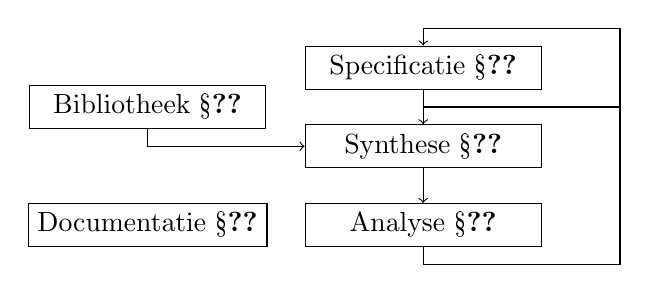
\begin{tikzpicture}[itm/.style={draw=black,rectangle,minimum width=3 cm,minimum height=0.5 cm}]
\node[itm] (Sp) at (0,0) {Specificatie \S\ref{ss:specificatie}};
\node[itm] (B) at (-3.5,-0.5) {Bibliotheek \S\ref{ss:bibliotheek}};
\node[itm] (Sy) at (0,-1) {Synthese \S\ref{ss:synthese}};
\node[itm] (A) at (0,-2) {Analyse \S\ref{ss:analyse}};
\node[itm] (D) at (-3.5,-2) {Documentatie \S\ref{ss:documentatie}};
\draw[->] (Sp) -- (Sy);
\draw[->] (B) |- (Sy);
\draw[->] (Sy) -- (A);
\draw (A) |- ++(2.5,-0.5) |- ++(-2.5,2);
\draw[<-] (Sp) |- ++(2.5,0.5) -- ++(0,-1);
\end{tikzpicture}
\caption{Typisch verloop van een digitaal ontwerp.}
\figlab{digitalDesignManagement}
\end{figure}
\subsection{Specificatie}
\label{ss:specificatie}
Een \termen{Specificatie} is een beschrijving van de functionaliteiten die van de hardware in kwestie gevraagd worden. In tegenstelling tot specificaties in bijvoorbeeld de informatica, is de \termen{interface} ook een onderdeel van de specificaties. De interface beschrijft hoe de hardware interageert met zijn omgeving. Deze omgeving is niet noodzakelijk de gebruiker die bijvoorbeeld toetsen indrukt en het scherm uitleest. Dit kan ook bijvoorbeeld de PCI\footnote{PCI: Peripheral Component Interconnect.} bus zijn waarmee met bijvoorbeeld een computer gecommuniceerd wordt. Dikwijls zijn initieel de specificaties onvolledig. De gaten in de specificaties worden dan ook opgevuld wanneer er zich problemen stellen in bijvoorbeeld de synthese. Specificaties zijn bijgevolg een iteratief proces. Dikwijls bevatten de specificaties ook reeds implementatiesbeslissingen die onnodige beperkingen opleggen aan het ontwerp. De beschrijving wordt ofwel in natuurlijke taal, wat soms dubbelzinnig is, of met behulp van een blokschema beschreven.
\subsection{Synthese}
\label{ss:synthese}
De \termen{Synthese} is niets anders dan de vertaling van de specificaties van een hoog en abstract naar een lager niveau. Hierbij dienen uiteraard concrete beslissingen genomen te worden over de implementatie. Zo kunnen de specificaties bijvoorbeeld vermelden dat $x$ en $y$ bij elkaar opgeteld moeten worden. De synthese moet dan een concrete implementatie voorstellen. Bijvoorbeeld een 16-bit ripple-carry adder met 2 registers. Synthese gebeurt meestal op verschillende niveaus. Zo worden op het laagste niveau componenten gebouwd. Dit zijn bijvoorbeeld de poorten maar ook bijvoorbeeld flipflops of multiplexers. Deze worden op een niveau hoger gebruikt om \termen{Register-Transfer-Level (RTL) Componenten} te bouwen. Deze RTL componenten zijn bijvoorbeeld optellers, schuifregisters en tellers. Schakelingen met deze componenten zijn dan \termen{Application Specific IC (ASIC) componenten}. Deze componenten vormen dan uiteindelijk de bouwblokken voor het systeem. Bij de systeemsynthese worden dan processoren, geheugens en de ASIC componenten gecombineerd. \figref{synthesisPyramid} toont de pyramide van synthese. Elk niveau combineert hierbij de componenten ge\"introduceerd op een niveau lager.
\begin{figure}[htb]
\centering
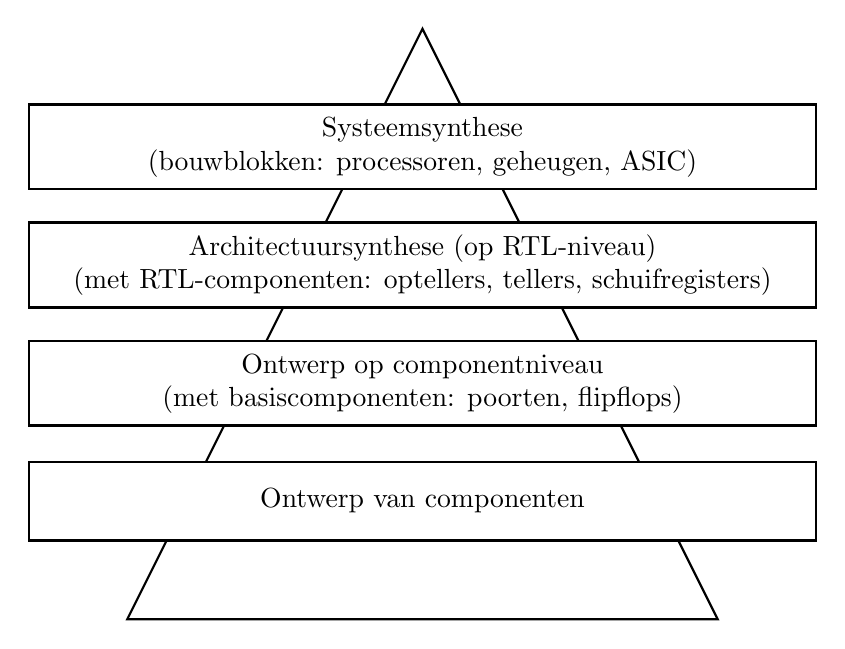
\begin{tikzpicture}[itm/.style={draw=black,thick,rectangle,fill=white,minimum width=10 cm,minimum height=1 cm}]
\draw[thick] (-3.75,0) -- (0,7.5) -- (3.75,0) -- cycle;
\node[itm] (LA) at (0,1.5) {Ontwerp van componenten};
\node[itm] (LB) at (0,3) {\begin{tabular}{c}Ontwerp op componentniveau\\(met basiscomponenten: poorten, flipflops)\end{tabular}};
\node[itm] (LC) at (0,4.5) {\begin{tabular}{c}Architectuursynthese (op RTL-niveau)\\(met RTL-componenten: optellers, tellers, schuifregisters)\end{tabular}};
\node[itm] (LD) at (0,6) {\begin{tabular}{c}Systeemsynthese\\(bouwblokken: processoren, geheugen, ASIC)\end{tabular}};
\end{tikzpicture}
\caption{De verschillende lagen bij de synthese.}
\figlab{synthesisPyramid}
\end{figure}
\subsection{Bibliotheek}
\label{ss:bibliotheek}
We dienen niet het volledige stuk hardware vanaf transistor of poortniveau te ontwerpen. Heel wat werk is dan ook al in het verleden door andere ontwerpers gedaan. Het hergebruiken van deze ontwerpen heeft dan ook heel wat voordelen:
\begin{itemize}
 \item De ontwerpen zijn meestal al door verschillende personen geoptimaliseerd. Het vinden van een nog optimalere implementatie is daardoor quasi onbestaand.
 \item Men streeft naar telkens hogere integratieniveaus waarbij soms volledige systemen op chip te verkrijgen zijn. Bovendien worden deze systemen telkens geavanceerder. Dit komt door de \termen{Wet van Moore}. Deze stelt dat elke 24 maanden het aantal transistoren op een chip verdubbelt.
 \item Vaak kan men componenten kopen die een bepaalde functie vervullen. Dit bespaart veel ontwerpwerk. Bovendien zijn deze componenten vaak veel goedkoper dan ze zelf te ontwerpen en te produceren. Bijvoorbeeld een 16 kB geheugen.
\end{itemize}
Er bestaan bibliotheken op elk syntheseniveau. Dus bijgevolg kan men tot op het niveau dat men zelf kiest putten uit de bibliotheken.
\subsection{Analyse}
\label{ss:analyse}
Na elke synthesestap is het belangrijk om te testen of aan de vereiste specificaties voldaan is. Dit wordt gedaan in de \termen{Analyse}. Niet alleen wordt hier getest of de implementatie de functionaliteit levert die gevraagd is, ook allerhande andere parameters worden in rekening gebracht:
\begin{itemize}
 \item Kostprijs: vaak wordt hier als metriek het aantal pinnen en de oppervlakte van de printplaat (PCB\footnote{PCB: Printed Circuit Board.}) gebruikt.
 \item Vermogengebruik: het vermogenverbruik wordt meestal berekend met de formule $C\cdot f\cdot V^2$ met als parameters:
 \begin{itemize}
  \item $C$ De oppervlakte van de chip. De oppervlakte is in de tijd toegenomen. In 1983 was een gemiddelde chip immers $0.25\mbox{ cm}^2$, in 2000 was dat ongeveer $4\mbox{ cm}^2$.
  \item $f$ De \termen{klokfrequentie}. De klokfrequentie is in de loop der tijd exponentieel gestegen. Met $1\mbox{ MHz}$ in 1983, en $1\mbox{ GHz}$ in 2000.
  \item $V$ De spanning die aan de chip geleverd wordt. De spanning is gedaald: van $5\mbox{ V}$ in 1983 tot $1.5\mbox{ V}$ ongeveer 17 jaar later.
 \end{itemize}
 \item Snelheid: de vertraging of \termen{doorvoer} (``\termen{throughput}''). Dit is het aantal resultaten per seconde.
 \item Testbaarheid: kunnen we alle fouten ontdekken met behulp van testvectoren?
\end{itemize}
\subsection{Documentatie}
\label{ss:documentatie}
Naast de hardware verlangt de klant meestal ook \termen{Documentatie}. Afhankelijk van het soort klant zal er andere documentatie vereist zijn. Indien we een volledig afgewerkt consumentenproduct maken, dienen we een handleiding voor de consument en de hersteller samen te stellen. Hierin beschrijven we in natuurlijke taal hoe de component aangestuurd kan worden. Indien we echter een component leveren, bijvoorbeeld een geheugenmodule zal men een handleiding maken met daarin de specifieke ontwerpdetails. Meestal zal ook intern binnen het bedrijf documentatie een vereiste zijn. Dit om de eventueel verdere ontwikkelingen te ondersteunen.
\subsection{Ontwerpen met CAD}
\termen{Computer Aided Design (CAD)} wordt vaak toegepast om een chip te ontwikkelen. Hierbij wordt met behulp van een computer een een speciaal softwarepakket meestal het volledige ontwerp begeleid. Een concreet voorbeeld hiervan is bijvoorbeeld \emph{KiCad} voor \emph{Linux}. Zoals andere CAD tools bevat \emph{KiCad} een project manager die de gebruiker door de verschillende stappen begeleidt, en een set tools die de gebruiker bij iedere stap de nodige ondersteuning bieden. Uiteraard ziet het ontwerp met een CAD-tool er gelijkaardig uit aan het ontwikkelingsproces op \figref{digitalDesignManagement}. De CAD-tools bieden echter meer mogelijkheden om ontwerpen al in een vroeg stadium te testen en te simuleren. \figref{digitalDesignManagementCad} toont het ontwikkelingsproces met behulp van een CAD-tool.
\begin{figure}[htb]
\centering
\begin{tikzpicture}[itm/.style={draw=black,rectangle,minimum width=4 cm}]
\node (Sp) at (0,0) {Specificatie};
\draw (Sp.north west) -- (Sp.north east) -- ++(0.15,-0.275) -- (Sp.south east) -- (Sp.south west) -- ++(-0.15,0.275) -- cycle;
\node (Sc) at (-1,-2.25) {Schema};
\draw (Sc.north west) -- (Sc.north east) -- ++(0.15,-0.275) -- (Sc.south east) -- (Sc.south west) -- ++(-0.15,0.275) -- cycle;
\node (V) at (1,-2.25) {VHDL};
\draw (V.north west) -- (V.north east) -- ++(0.15,-0.275) -- (V.south east) -- (V.south west) -- ++(-0.15,0.275) -- cycle;
\draw (-2,-1.25) rectangle ++(4,-1.5);
\draw (0,-1.25) node[anchor=north]{Ingave ontwerp};
\draw[->] (Sp) -- (0,-1.25);
\node[itm] (Sy) at (0,-4) {Synthese};
\draw[->] (0,-2.75) -- (Sy);
\node[itm] (Fs) at (0,-6) {Functionele Simulatie};
\draw[->] (Sy) -- (Fs);
\node[draw,shape aspect=2,diamond] (O) at (0,-8) {Ontwerp OK?};
\draw (O.south) node[anchor=north west]{Ja};
\draw (O.west) node[anchor=south east]{Nee};
\draw[->] (Fs) -- (O);
\node[itm] (Fo) at (6,-2) {Fysisch ontwerp};
\draw[->] (O.south) |- ++(3,-0.5) |- (Fo.west);
\node[itm] (St) at (6,-4) {Simulatie tijdsgedrag};
\draw[->] (Fo) -- (St);
\node[draw,shape aspect=2,diamond] (T) at (6,-6) {Tijdsgedrag OK?};
\draw (T.south) node[anchor=north west]{Ja};
\draw (T.west) node[anchor=south east]{Nee};
\draw[->] (St) -- (T);
\draw (T) -- ++(-3,0);
\draw (3.5,-6) |- (-3,-10) -- (-3,-8);
\draw (O) -| (-3,-0.625) -- ++(3,0);
\node[itm] (C) at (6,-8) {Chipconfiguratie};
\draw[->] (T) -- (C);
\end{tikzpicture}
\caption{Digitaal ontwerpen met CAD.}
\figlab{digitalDesignManagementCad}
\end{figure}
\section{Taalgebaseerd hardware ontwerp: VHDL}
\seclab{vhdl}
Zoals reeds vermeld werd op \figref{digitalDesignManagementCad}, wordt \termen{VHDL} veel gebruikt om schakelingen in te voeren in een computersysteem. VHDL is de afkorting van \termen{VHSIC Hardware Description Language}. Hierbij staat VHSIC voor \termen{Very High Speed Integrated Circuit}. VHDL is een programmeertaal waarmee men het gedrag van digitale circuits probeert te beschrijven. De taal biedt mogelijkheden aan om op een eenduidige manier het gedrag van een circuit te specifi\"eren op RTL niveau. Daarnaast is de taal erg nuttig om simulaties te draaien, synthese uit te voeren (VHDL software is meestal in staat om zelf effici\"ente implementaties voor te stellen) en documentatie te genereren. VHDL is gestandaardiseerd bij de IEEE\footnote{IEEE: Institute for Electrical and Electronics Engineers.}. De eerste versie van VHDL is VHDL-87, gestandaardiseerd onder IEEE 1076. In 1993 werd de tweede versie, VHDL-93 uitgebracht in IEEE 1164. Sinds 2002 bestaat er ook een derde versie die nog niet gestandaardiseerd is. Deze standaarden omvatten echter uitsluitend de syntax. De implementatie van de VHDL compiler is volledig vrij. Er is dan ook concurrentie tussen VHDL compilers in features om de meest effici\"ente implementatie te kunnen voorstellen.
\subsection{Alternatieven en uitbreidingen}
\paragraph{VHDL-AMS}Een uitbreiding op VHDL is \termen{VHDL Analog and Mixed Signals (VHDL-AMS)}. Hierbij worden niet alleen digitale maar ook analoge signalen beschouwd. VHDL-AMS kan dus als een superset van de orginele VHDL beschouwd worden. Bovendien wordt met continue tijd gerekend in plaats van de door VHDL gebruikte discrete tijdstippen. Dit werd ge\"implementeerd door een set algebra\"ische en differenti\"ele vergelijkingen. Hoewel het in 1999 door de IEEE gestandaardiseerd werd, is VHDL-AMS sinds zijn oorsprong in 1993 nooit echt doorgebroken.
\paragraph{Verilog}De concurrent van VHDL is \termen{Verilog} (IEEE 1364). Verilog is erg populair in de Verenigde Staten maar is nooit echt doorgebroken in Europa. Beide talen stammen ook uit andere taalfamilies met andere paradigma's. Terwijl \verb+VHDL+ eerder lijkt op \verb+Ada+, is \verb+Verilog+ meer verwant met \verb+C+. Ondanks de concurrentie lijkt geen van beide talen het pleit te kunnen beslechten. Of zoals D. Pellerin \& D. Taylor het verwoorden in ``VHDL Made Easy!''\cite{pellerin1997vhdl}:
\begin{quote}
Both languages are easy to learn and hard to master. And once you have learned one of these languages, you will have no trouble transitioning to the other.
\end{quote}
\paragraph{PLD talen}
Talen zoals Abel en Palasm zijn zogenaamde \termen{PLD talen}\footnote{PLD: programmable Logic Device, zie \ref{sss:pld}.}. Deze talen specifi\"eren schakelingen op het niveau van de poorten en dit slechts voor een speciale technologie. Deze talen hebben bijgevolg ook een ander objectief. Waar VHDL net bedoeld is om zich met de details bezig te houden, en de gebruiker met de grote lijnen, zijn PDL talen bedoelt om te implementeren op deze lagere niveaus.
\subsection{Voordelen}
VHDL wordt hoofdzakelijk in de industrie gebruikt omwille van zijn overdraagbaarheid. VHDL is immers een standaard die door allerhande programma's gehanteerd wordt. Elk van deze programma's kunnen heel diverse toepassingen hebben. Op die manier kan een stuk VHDL eerst gesimuleerd worden met het ene programma, daarna gesynthetiseerd met een ander, om bijvoorbeeld geanalyseerd te worden met een derde programma. Deze programma's kunnen bovendien afkomstig zijn van verschillende fabrikanten. Hierdoor kunnen fabrikanten zich ook toespitsen op \'e\'en kant van het ontwerp zonder dat er compatibiliteitsproblemen ontstaan.
\paragraph{}
Daarnaast is VHDL ook interessant om complexe schakelingen op een hogere abstractieniveau te beschrijven. Zo kan men een schakeling die vaak terugkomt groeperen in een bepaalde module. Repetitieve structuren dienen slechts \'e\'enmaal beschreven te worden, maar kan men eindeloos blijven gebruiken.
\paragraph{}
VHDL maakt het ook mogelijk om de gebruiker te laten ontwerpen los van de eigenlijke implementatie. Zo dient de gebruiker alleen te specificeren dat twee getallen opgeteld moeten worden. Het is dan aan het programma om de componenten te selecteren die dat op de beste manier doen (qua kosten, snelheid,...).
\paragraph{}
Tot slot zorgt VHDL er ook voor dat een ontwerp makkelijk te parametriseren valt. Indien de ontwerper niet zeker is van de woordlengte van zijn processor kan hij deze in een parameter onderbrengen. Als later blijkt dat de woordlengte groter moet zijn, kan met een eenvoudige verandering van de parameterwaarde het volledige model aangepast worden.
\subsection{Nadelen}
Naast de reeks opgesomde voordelen heeft VHDL ook enkele belangrijke nadelen. Zo is het een eenvoudig te leren taal, maar de taal echt beheersen vraagt heel wat geduld. Dit komt door een deel door de niet eenvoudige syntax. Een ander probleem is dat heel wat software afwijkt van de gestandaardiseerde versies. Er bestaan dan ook onnoemelijk veel VHDL ``dialecten'' waardoor sommige features die aan de taal werden toegevoegd slechts op bepaalde softwarepakketten werken.
\paragraph{}
Een ander nadeel is dat de taal nogal langdradig is. Bij complexe circuits zullen de groeperingen zeker hun effect hebben, maar om kleine schakelingen te realiseren is nogal veel code nodig.
\paragraph{}
Een probleem met code in het algemeen is dat het erg onoverzichtelijk is. Een eenvoudig blokschema is nog altijd overzichtelijker omdat mensen nu eenmaal grafisch sterker zijn. Pas bij grote complexe schakelingen verliest het visuele zijn kracht en zal een stuk code als doeltreffender worden aanzien.
\paragraph{}
Het feit dat VHDL redelijk uitgebreid is, brengt bovendien allerhande nadelen met zich mee. Alle extra features voor bijvoorbeeld tijdsgedrag simulaties dienen immers in de taal beschreven te kunnen worden. Bijgevolg worden sommige taalconcepten hierdoor hopeloos moeilijker gemaakt.
\subsection{Beperkingen}
Naast de voor- en nadelen heeft VHDL ook enkele beperkingen. Zo is VHDL slechts tot op zeker niveau automatisch synthetiseerbaar. Hierbij ondersteunt elke fabrikant van VHDL een verschillende subset. Het tweede grote nadeel is dat slechts de syntax en de semantiek van VHDL gestandaardiseerd is. Niet hoe de code geschreven moet worden. Dit houdt in dat eenzelfde gedrag op tientallen verschillende manieren beschreven kan worden. Dit zorgt er ook voor dat elk programma dat VHDL leest de code op een andere manier kan implementeren. Het gevolg is dat de codestijl, die in grote mate bepaalt hoe de code ge\"implementeerd zal worden, variabel is. In het ene programma kan een bepaalde code tot de meest optimale implementatie leiden, terwijl een ander programma met dezelfde code slechts een standaardimplementatie kiest. Men moet dus eerst heel wat ervaring opdoen met een programma alvorens men weet hoe men de code moet schrijven zodat deze een effici\"ente implementatie kiest.
\subsection{Concepten (entiteiten en architectuur)}
Na de voor en nadelen besproken te hebben, is het tijd voor een voorbeeld waarmee we de verschillende concepten zullen duidelijk maken. We ontwerpen een schakeling zoals op \figref{vhdl-example}. Hierbij willen we een schakeling ``test'' ontwerpen. Deze schakeling krijgt drie 8-bit ingangen (\texttt{In1}, \texttt{In2} en \texttt{In3}). Als uitgangen zijn er twee bits (\texttt{Out1} en \texttt{Out2}). \texttt{Out1} geeft 1 terug indien \texttt{In1} en \texttt{In2} aan elkaar gelijk zijn. Analoog geeft \texttt{Out2} 1 terug indien \texttt{In2} en \texttt{In3} gelijk zijn. Om deze vergelijker te bouwen werken we bijgevolg met een hi\"erarchisch schema. Waarbij we \texttt{Comp} op een andere plaats implementeren.
\importtikzfigure{vhdl-example}{Voorbeeldcircuit voor VHDL code.}
\paragraph{}We zullen eerst \texttt{Comp} implementeren in VHDL. De code hiervoor staat in \vhdlref{comp}. Als we de code goed bekijken onderscheiden we twee belangrijke delen \vhdltermen{entity} en \vhdltermen{architecture}.
\paragraph{Entity}
Het \texttt{entity} gedeelte beschrijft de zogenaamde ``\termen{blackbox}'' ofwel de interface. Hierdoor is VHDL in staat een blokje te tonen met de juiste in en uitgangen. Zoals we zien bevat de beschrijving het \vhdltermen{port} commando. Het \texttt{port} commando specificeert dan de in- en uitgangen. Dit doet men door eerst de namen van de in- of uitgangen te vermelden. Vervolgens plaatst men het token \vhdltermen{in} of \vhdltermen{out} om te specificeren of het om een in- of uitgang gaat. Merk dus op dat elke geleider naar de component een expliciete richting heeft. Vervolgens duidt men het type van de in- of uitgang aan. Logischerwijs bevat dit het token \vhdltermen{bit}. Een bit is niets anders dan \'e\'en lijn. Meestal echter willen we verschillende lijnen samennemen. In dat geval duiden we dit aan met een \vhdltermen{bit\_vector}, een bitvector is dus niets anders dan een lijst van geleiders naar het blok. Het is handig verschillende geleiders samen te nemen, dit maakt de code overzichtelijker. Indien bijvoorbeeld de lengte van A gewijzigd moet worden kost dit slechts een minimale ingreep.
\paragraph{Architecture}
De concrete werking wordt beschreven in het \texttt{architecture} gedeelte. Dit beschrijft het gedrag van de component op RTL-niveau. VHDL is in staat met de gegeven beschrijving in de \texttt{architecture} omgeving een implementatie op poortniveau te bouwen. Verder dient ook opgemerkt te worden dat \'e\'en \texttt{entity} verschillende \texttt{architecture}s kan hebben.\footnote{Vandaar dat we onze architectuur de naam \texttt{Behav1} noemen.}. Uiteraard moeten al deze \texttt{architecture}s met dezelfde interface werken.
\begin{vhdlcode}
\centering
\begin{lstlisting}
-- 8-bit comparator
--
entity Comp is
  port(	A,B: in bit_vector(0 to 7);
	EQ: out bit);
end entity Comp;

architecture Behav1 of Comp is
begin
  EQ <= '1' when (A=B) else '0';
end architecture Behav1;
\end{lstlisting}
\caption{8-bit comparator.}
\label{vhdl:comp}
\end{vhdlcode}
\paragraph{Component} Nu we een comparator component gebouwd hebben, zullen we deze component importeren in ons testcircuit. Hiervoor gebruiken we code beschreven in \vhdlref{test}. Dit bestand deelt dezelfde structuur als de structuur in \vhdlref{comp}: een \texttt{entity} en \texttt{architecture}. Dit wijst er dus op dat we componenten hi\"erarchisch kunnen gebruiken. We bemerken echter een nieuw token: \vhdltermen{component}. \texttt{component} is een virtuele verwijzing naar een andere entiteit. Wat die entiteit is laten we in de code nog in het midden. Het enige wat we moeten doen is de interface van deze component specificeren. Later zullen we dan in de configuratie (\vhdlref{testConfig}) een binding voorzien tussen ons virtuele component \texttt{comparator} en onze gedefinieerde entiteit \texttt{comp}. Verder merken we ook op dat in het \texttt{architecture} gedeelte eenmaal we de \texttt{component} interface gedefinieerd hebben, we er instanties van kunnen aanmaken. Zo maken we twee instanties aan: \texttt{Comp1} en \texttt{Comp2}. Vervolgens dienen we nog de verbindingen tussen de entiteit \texttt{test} en deze instanties te leggen. Dit doen we met het token \vhdltermen{map}. Hierbij mappen we de variabelen uit \texttt{entity Test} (\texttt{In1}, \texttt{In2}, \texttt{In3}, \texttt{Out1} en \texttt{Out2}) op de in- en uitgangen van het \texttt{component Comparator} (\texttt{X}, \texttt{Y} en \texttt{Z}). Hierbij dient dus opgemerkt te worden dat we het gedrag van \texttt{Test} specificeren aan de hand van reeds gedefinieerde entiteiten. Tot slot dient ook opgemerkt te worden dat in tegenstelling tot klassieke programmeertalen alle componenten tegelijk werken. Het is dus niet zo dat bij het uitrekenen van \texttt{Test} eerst \texttt{Comp1} en dan \texttt{Comp2} uitgerekend zal worden.
\begin{vhdlcode}
\centering
\begin{lstlisting}
-- Component Test met 2 comparatoren
--
entity Test is
  port(	In1,In2,In3: in bit_vector(0 to 7);
	Out1,Out2: out bit);
end entity Test;

architecture Struct1 of Test is
component Comparator is
  port(	X,Y: in bit_vector(0 to 7);
	Z: out bit);
end component Comparator;
begin
  Comp1: component Comparator port map (In1,In2,Out1);
  Comp2: component Comparator port map (In2,In3,Out2);
end architecture Struct1;
\end{lstlisting}
\caption{Voorbeeldcode.}
\label{vhdl:test}
\end{vhdlcode}
\paragraph{Configuration} We moeten nu \texttt{Comparator} met de entiteit \texttt{Comp} binden. Dit doen we in een \vhdltermen{con\-fig\-ura\-tion} omgeving. Deze configuratie wordt beschreven in VHDL-code \ref{vhdl:testConfig}. Zoals we zien kunnen we opnieuw verschillende \texttt{configuration}s aanmaken en deze een aparte naam geven. Op die manier kunnen we dus de feitelijke implementatie snel wijzigen. Verder dienen we ook te vermelden welke entiteit we zullen configureren (\texttt{Test}) en om welke architectuur het gaat (\texttt{Struct1}). Vervolgens kunnen we per instantie aangeven welke entiteit we gebruiken. Dit doen we door het token \vhdltermen{use entity}. Ook specifi\"eren we de \texttt{architecture} die we zullen gebruiken van deze \texttt{entity}. Vervolgens mappen we opnieuw met behulp van \texttt{map} de in- en uitgangen van de entiteit op het virtuele \texttt{component}.
\begin{vhdlcode}
\begin{lstlisting}
-- Configuratie: definieer koppeling component met een
-- bepaalde architectuur van een entiteit
--
configuration Build1 of Test is
  for Struct1
    for Comp1: Comparator use entity Comp(Behav1)
      port map (A => X, B => Y, EQ => Z);
    end for;
    for Comp2: Comparator use entity Comp(Behav1)
      port map (A => X, B => Y, EQ => Z);
    end for;
  end for;
end configuration Build1;
\end{lstlisting}
\caption{Configuratie van de voorbeeldcode.}
\label{vhdl:testConfig}
\end{vhdlcode}
\subsection{Gelijkenissen en verschillen met klassieke programmeertalen}
VHDL lijkt in sommige opzichten een beetje op programmeren in klassieke programmeertalen zoals \texttt{Java} en \texttt{C++}. Immers kunnen we de ingangen als parameters bij een methode zien. De methode zelf fungeert ook als een interface die duidelijk maakt welke types er ingevoerd moeten worden, en welke uitvoer verwacht mag worden, zonder de feitelijke implementatie te tonen. We zouden bovendien elk component die we in een circuit gebruiken kunnen zien als een functie-oproep naar de functie van het bijbehorende component. Deze vergelijking heeft echter enkele anomalie\"en.
\begin{itemize}
 \item \termen{Gelijktijdigheid} (``\termen{Concurrency}''): Alle hardwarecomponenten werken in parallel dit in tegenstelling tot klassieke talen waarin alles sequentieel wordt uitgevoerd.
 \item \termen{Tijdsconcept}: Alle hardware werkt continu en houdt nooit op met werken. Bovendien zal bij een simulatie de tijd uiteraard niet de re\"ele tijd zijn.
 \item \termen{Datatypes}: VHDL heeft nood aan typische hardware-types zoals bitvectoren, getallen met geparametriseerde grootte,... Dit terwijl klassieke talen meestal proberen abstractie te maken van dit hardwareniveau.
\end{itemize}
